\documentclass[a4paper,10pt]{article}
\usepackage{a4wide}
\usepackage[utf8]{inputenc}
\usepackage{graphicx}
\usepackage{hyperref}
\usepackage{natbib}


% Title Page
\title{Manual for occup\_3d\_ext and its auxiliary utilities}
\author{Johann Weber}



\begin{document}
\parindent 0em
\bibliographystyle{plainnat}
\maketitle

%\begin{abstract}
%This is the documentation for the 3D radiative transfer program
%\texttt{occup\_3d\_ext}.
%\end{abstract}

\tableofcontents

\section{Introduction}
\label{sec:intro}
\texttt{occup\_3d\_ext} is a 3D radiative transfer code able to account for 
atomic gas. It currently considers hydrogen, helium and the ionization stages  
I to IV of carbon, nitrogen, oxygen, neon and sulfur. Implementation details 
have been described in detail in \cite{Weber2013} and \cite{Weber2015}. 
In this manual we will focus on the usage of the program. 

\section{Requirements}
\texttt{occup\_3d\_ext} has been developed in Fortran 2003, but the only 
Fortran 2003 specific features used so far are the  calls to  the subroutine 
\texttt{get\_command\_argument}, the function \texttt{command\_argument\_count} 
(both of these subprograms are related to the handling of command line options) 
and the \texttt{flush} statement. Thus each Fortran 95 compatible compiler 
that additionally  supports these extensions may be able to generate the 
\texttt{occup\_3d\_ext} program.

The program has been tested with the Intel Fortran  
compiler\footnote{\url{http://software.intel.com/en-us/fortran-compilers}} 
(Versions later than 9) and the GNU Fortran compiler \texttt{gfortran} which is
freely available for all relevant platforms. 
Details about \texttt{gfortran} can be found at\\
\url{http://gcc.gnu.org/wiki/GFortran}.

\texttt{occup\_3d\_ext}  can in principle be compiled for 32 bit systems, but 
large simulations (e.g including $101^3$ grid cells) that account for the 
ionization structure of metals and/or the escape fractions will only run on 64 
bit machines with a sufficient amount of RAM.

The program has been tested on Linux and Windows 7. As there no operating system 
dependent calls, it is likely to work on other operating systems like OS\,X or 
BSD-type unixes. 

The only external dependency of the program is the \texttt{LAPACK} library. This 
may be available from your compiler supplier, either included with your compiler 
(as it is the case for Intel Fortran Version 11 or later) or as a separate  
package (e.g. for the older versions of Intel Fortran). Alternatively it is 
possible the download the reference implantation from NIST available from\\ 
\url{http://www.netlib.org/lapack/index.html}.\\ This version may however be 
slower than the platform-specific versions of the compiler versions. 
\texttt{LAPACK} is also provided in the repositories of the major Linux 
distributions.

In order to utilize parallelization on multi-processor machines, 
\texttt{occup\_3d\_ext} relies on OpenMP\\ 
(\url{http://http://openmp.org/wp/})\\ directives (see also 
Appendix~\ref{appendix:performance}). On compilers that do not 
support OpenMP, \texttt{occup\_3d\_ext} processes will not take profit form 
multi-core CPUs\footnote{Of course it is still be possible to run several 
instances  of \texttt{occup\_3d\_ext} (i.e. different simulations) in 
parallel.}. Using an OpenMP-compatible compiler is therefore strongly 
recommended. OpenMP is supported by most of the recent Fortran compilers. 
\texttt{gfortran} supports OpenMP in version 4.2 or later. 

To compile the documentation a \LaTeX\ compiler is required. Both \texttt{latex} 
and \texttt{pdflatex} can be used, but hyperlinks and cross-references are only 
supported if either \texttt{pdflatex} is used or the Postscript file 
generated by \texttt{latex} and \texttt{dvips} is converted 
into a PDF file afterwards. The documentation requires the latex packages 
\texttt{a4wide}, \texttt{hyperref}, \texttt{inputenc}, \texttt{graphicx}, and 
\texttt{natbib} to be installed.

\section{Compiling}
Provided with the source code is a Makefile.
You will probably have to modify the Makefile to
set the correct library paths, commands and compiler options.

The Makefile currently includes several build targets:
\begin{itemize}
\item \texttt{make binary} Creates the binary file using Intel Fortran.
\item \texttt{make binary\_gfortran} The system is built  using the GNU Fortran 
compiler. This option may be removed in the future. It is recommended to modify 
the variables of the \texttt{binary target} such that they meet your build 
environment.\item \texttt{make all} This option currently corresponds to 
make\_binary (using the Intel Compiler)\footnote{Note that the \LaTeX sources of 
this document are no longer contained in the same directory as
the Fortran source files, but instead in the directory 
\texttt{\$ug/manual\_3d\_ext} of the \texttt{Doc} module. This document can
be rebuilt by calling
\texttt{latex manual.tex}
or 
\texttt{pdflatex manual.tex}
three times (which is necessary for the generation of the correct citations and 
references). The hyperlinks within this document only work in PDF files, but not 
in Postscript of DVI files.} \item \texttt{make clean} Removes all but the 
source files.
\end{itemize}

There also exists a Visual Studio 2005 project file (adapted to Version 9 of  
the Intel Fortran compiler) in the directory\\
\texttt{WMbasic\_IVF\textbackslash Occup}
to create \texttt{occup\_3d\_ext},
 wheras the VS 2005 projects to create the auxiliary programs are
located in\\
\texttt{WMbasic\_IVF\textbackslash Utilities\textbackslash Occup\_3d\_ext\_utils}.\\
Like the Makefile, these will probably have to be modified in order the run on 	
your system.

If your development environment is neither Visual Studio nor does  include the 
\texttt{make} command  you have to 
care about the correct order of the compilation and linking processes yourself.

There is no installation that copies the compiled program and the documentation  
to an ``usual'' location in the file system like \texttt{/usr/local/bin} or 
\texttt{/usr/share/doc} or sets the \texttt{\$PATH} (MS Windows: 
\texttt{\%Path}). If setting the paths is desired, this has to be done manually 
by the user. The only environment variables  that are evaluated are the 
variables that control the behavior of OpenMP. The environment variable 
\texttt{\$OMP\_NUM\_THREADS} is an integer, which determines the number of 
parallel OpenMP threads. It should have the same value as the 
\texttt{\hyperref[opt:numthreads]{num\_threads}} variable in the input file. 
If the values differ, the program will still run correctly, but the performance 
will be poor. So far the have been no benchmarks of the effects of the other 
OpenMP-related environment variables.   

\section{Testing the program}
The \texttt{testcases} directory contains the input files required to test the 
program after it has been compiled. The test case represents a homogeneous 
H\,II region surrounding a a 40 kK dwarf star. Both the nebular and the stellar 
metallicity corresponds to the solar value (The values for the "solar 
metallicity" correspond to the ones in \citealt{Asplund2009}, the properties of 
the corresponding stellar model are decribed in \citealt{Weber2015}). Simulated 
is one octant of the H\,II region. The input files are
\begin{itemize}
\item \texttt{input\_values}: This file contains the namelist with the  
simulation parameters.
\item \texttt{sources.txt}: File containing the position, the radius, the  
lifetime and the name of the file with the SED of the source
\item \texttt{MERGESPEC}: File containing the stellar SED.
\end{itemize}
The structure of the files will be explained in detail in the next section.

The program is finally run by\\
\texttt{\textit{<Path to executable>}/occup\_3d\_ext < input\_values} . \\
The execution time for the testcase is approximately 40 minutes for a single  
thread on a Intel Xeon (Core 2 Architecture) when the Intel Fortran Compiler 
V~13 is used and the optimizations are activated. 
For convenience, there exist scripts that automatically run the test case and  
prepare the output files for \texttt{gnuplot} 
(using \texttt{\hyperref[util:radiusbench]{radiusbench}}), 
which is then applied to generate plots that show the abundances  and the  
temperature as a function of the distance from the source.
The UNIX script is located in the \texttt{testcases/ref\_3d\_ext}  subdirectory 
and called \texttt{run\_ext\_3d\_testcase}. The Windows batchfile, called  
\texttt{run\_ext\_3d\_testcase.bat}, is located in 
\texttt{WMbasic\_IVF\textbackslash Utilities\textbackslash bat\_local\_use} .
The names of the output files of the scrips have the structure  
\texttt{comparison-\textit{xx}.ps}, the reference files are called 
\texttt{reference-\textit{xx}.ps}. Here \textit{xx} is either the
name of the corresponding chemical symbol or \texttt{temp} in the case of the	 
file showing the temperature structure.


\section{File formats}
\label {sec:fileformats}
\subsection{The main input file (input)}
\label{file:main}
In the main input file,  the variables which specify the behavior of the 
program  are set. The format of the corresponds to a Fortran namelist. A sample 
file 
called \texttt{input\_values}\footnote{As the file is passed to the program via 
standard input, the name of the file does not matter} is provided with the 
source code.

The file starts with the line\\
\texttt{\&input\_values}\\

Then the options and simulation parameters are given their values via pairs of 
the form \textit{variable} = \textit{value},
where each of the assignments is followed by a comma and, if desired to improve	 
readability of the input file, a "\texttt{\&}", followed by a newline. More 
information about namelists can be obtained, for instance, from  
\url{http://de.wikibooks.org/wiki/Fortran:\_Fortran\_95:\_Ein-\_und\_Ausgabe} 
(in German). Note that even the last assignment 
has to be followed by a comma. The notation of the values corresponds to the 
notation that is used in Fortran source code. The file is terminated by a slash.

If no value is assigned to a variable in the input file, the default values  
will be used. For some variables  there are no default values, which may lead 
to undefined behavior. However, these variables are only evaluated if certain 
options are switched on. For details see the description of 
the corresponding options in Sect. \ref{sec:inputfile}.

\subsection{The file describing the sources (input)}
\label{file:sources}
The sources of ionization are usually (but see below) described in a separate 
file, with the default  name \texttt{sources.txt}. A sample is provided with 
the source code. In the 
main input file the name of input file for the sources of ionization can be 
changed by modifying \texttt{\hyperref[opt:sourcefilename]{source\_filename}}.
The structure of the file is as follows:
\begin{itemize}
\item The first line of the file can contain an arbitrary 
text/comment/explanations and is not evaluated.
\item The second line contains the (integer) number of sources.
\item The third line is a comment again.
\item The fourth line has the structure\\
$x$ $y$ $z$ $radius$ $spectrum$ $start$ $stop$\\
Here the integer value $x$ represents the $x$-index of the cell the source is 
located in. The $x$ values have to be within the interval $[-x\_max : 
+x\_max]$. $y$ and $z$ represent the indexes in the other dimensions. $radius$ 
is the radius of the source in solar radii. If the source is not a spherical 
object, a representative radius has to be chosen. $spectrum$ defines a file, 
which contains 
the description of the SED of the ionizing source. 
\texttt{occup\_3d\_ext} reads files, whose formats corresponds the format of 
the \texttt{MERGESPEC} files that are a output of the WM-Basic code, cf. \cite 
{Pauldrach2001} and \cite{Hoffmann2012}. It 
\texttt{mergespec=.false.}, the program uses the  format, that has been used in 
previous version of \texttt{occup\_3d\_ext}. The file \texttt{ps4e+4.txt} that 
is included with the source code (but not used in the default testcase) is in 
the format of the  older  versions. These file start with 16 
lines that are either empty or may be used for comments. The next 2001 lines 	
contain two columns, where the first columns is the wavelength in \AA{}, the 
second column is the corresponding Eddington flux $H_\nu$ in 
$\mathrm{erg\,s^{-1}\,sr^{-1}\,cm^{-3}}$. It is not currently possible to use 
both types of file formats in the same simulation. 
\item For each source, there follow two lines where the 
first one is a comment and the second one describes the source in the format 
described above. 
\item If the option \hyperref[opt:nosourcefilename]{no\_source\_filename} is 
set to \texttt{.true.}, the sources are not read from a separate file, but from 
the same file that contains the namelist
\texttt{input\_values}, for the setup of the simulation runs.
\end{itemize}

\subsection{The file describing the density structure (input)}
\label{file:density}
If \texttt{\hyperref[opt:readfromfile]{read\_from\_file}=.true.} the user has to 
specify the density structure of the gas in a file, whose name is specified in 
the option \texttt{ifrit\_filename}\footnote{IFrIT is a visualization program 
by Nickolay Gnedin, which concentrates on the visualization of ionization 
fronts and density structures. It can be obtained for free from 
\url{https://sites.google.com/site/ifrithome/} and is available for Windows  and 
for Unixes. 
On the homepage one can also find the documentation of the program
and its file formats.}. 
In the first line the dimension of the simulated volume in units of grid cells  
is set. Note that the absolute size of the simulation volume additionally 
depends on the option \texttt{\hyperref[opt:lcell]l\_cell}, which specified the 
length of an edge of a single grid cell in parsec. Because of the symmetry of 
the coordinate system -- the cell with the coordinates $(0,0,0)$ 
is located in the center of the simulated volume -- the first line has the form

$2\times\mathtt{x_{max}}+1 ~$  $2\times\mathtt{y_{max}}+1 ~$
$2\times\mathtt{z_{max}}+1~~$ .
For example, if $\mathrm{x\_{max}}=20$, $\mathrm{y\_{max}}=30$ and 
$\mathrm{z\_{max}}=40$, then the first line is

\texttt{41 61 81}

The remaining lines contain in their first row the total hydrogen number 	
density and in their second row the number density of neutral hydrogen in 
$\mathrm{cm^{-3}}$ at the beginning of the simulation. The order of the grid 
cells is optimized for Fortran, i.e. the loop over the different 
$z$-values is the outermost loop and the loop over the $x$-values is the  
innermost loop. The file may contain no empty lines or comments and end with a 
newline character.
 
Note that it is not possible to set the initial conditions for the ionization  
structures of elements other than hydrogen. To do so the 
\texttt{\hyperref[sec:commandlineoptions]{-resume} }
command line option has to be used.

\subsection{The files describing the ionization structure (output)}
\label{file:ionization}
The structure of the files which describe the ionization is compatible to IFrIT.
In the first line the dimension of the volume is specified in 
Sect.~\ref{file:density}. For each grid cell, the first $n$ columns contain the 
number densities (in units of $\mathrm{cm^{-3}}$ ) for the density of the ions 
$\mathrm{E}$ (i.e. neutral atoms of an element $\mathrm{E}$) to 
$\mathrm{E}^{+n-1}$. The last column contains the total number density of the 
atoms/ions belonging or the corresponding element. Currently supported are  
hydrogen ($\mathrm{H}$ and $\mathrm{H}^+$), helium  ($\mathrm{He}$, and 
$\mathrm{He}^+$ and $\mathrm{He}^{2+}$), and the most important metals 
$\mathrm{C}$, $\mathrm{N}$, $\mathrm{O}$, $\mathrm{Ne}$, $\mathrm{S}$
and $\mathrm{Ar}$.

Additionally a file with the suffix \texttt{.e.txt} is written which contains 
the electron number density in $\mathrm{cm^{-3}}$.

\textit{There currently exist problems to visualize the output  
data with newer Linux-Versions of IFrIT if the locale is set to German or 
another language that uses commas a decimal delimiters. The problem can be 
solved by setting the environment variables \texttt{LANG=en\_US.UTF-8} and
\texttt{LC\_NUMERIC=en\_US.UTF-8}. The Windows version of IFrIT seems to be 
unaffected by this problem.}


\subsection{The files describing the thermal energy and the 
temperature (output)}
\label{file:temperature}
If \texttt{\hyperref[opt:computetemperature]{compute\_temperature}=.true.}  
files are written that describe the temperature structure of the simulated 
file. 

\begin{itemize} 
\item The file with the suffix \texttt{.temp.txt} is an IFrIT compatible file 
that contains in its first column the temperature of the cells before the past 
timestep in K, in its second column the temperature after the past timestep in 
K, an in its third column the mean value of the temporal derivative of the 
temperature $\frac{\mathrm{d}T}{\mathrm{d}t}$ in units of $\mathrm{K/yr.}$ 
\item The IFrIT file with the suffix \texttt{.energy.txt} contains in its only 
column the density of the thermal energy in units of $\mathrm{erg~cm^{-3}}$. 
\item The files with the ending \texttt{.\textit{xx}.heatcool.txt}, where 
\texttt{xx} is 
the name of the element contain the heating and the cooling rates per element. 
In the IFrIT compatible files the first column contains the heating rates, the 
second column the cooling rates, and the third column the difference between 
the heating and the cooling rates. The used units are $\mathrm{erg~s^{-1} 
cm^{-3}}$.
\end{itemize}
  
\subsection{Logging of the timesteps in \texttt{time.txt} (output)}
\label{file:time}
In the file \texttt{time.txt} the timesteps are logged. The file format is not  
compatible to IFrIT, as the simulated time is a global property of the system 
and not a property that differs from cell to cell. The first column contains 
the length of the past timestep in years, the second column the total simulated 
time since the start of the simulated process and the third the counter for the 
timesteps. 
The fourth column is the wallclock time required per iteration cycle, the fifth 
column the CPU time per iteration cycle. A comparison of the two latter values 
indicates how well the code is parallelized (see 
Sect.~\ref{appendix:performance}).
If  
\texttt{\hyperref[opt:traceexpansion]{trace\_expansion}=.true.,} the sixth 
column contains the redshift at the given time and the counter for the 
timesteps is written in the seventh column.  

The second to last line contains the wall-clock time required to compute the 
past iteration step, the last line the amount of CPU time needed. Both values 
are given in seconds. Note that in some cases there might be negative value for 
the wall-clock time. The reason in an integer overflow affecting the Fortran 
routine \texttt{system\_clock}. As this affects only a small fraction of all 
timesteps, \texttt{time.txt} is still useful to analyze the performance. 
However, in a numerical data analysis program that works with data from 
\texttt{out.txt}, these effects have to be accounted for. It is not clear yet, 
how this problem can be fixed in a portable way  in the Fortran source code.

If the program program is restarted using the \texttt{-resume} command line  
option, the currently a new \texttt{time.txt} file such that the log for the 
previous timesteps is deleted. A workaround is to rename the older version 
before restarting the program. For more details about restarting a program, see 
Sect. \ref{sec:commandlineoptions}.

\subsection{Results for the escape fractions (output)}
If 
\texttt{\hyperref[opt:owriteescapefraction]{o\_write\_escape\_fraction}=.true.} 
the escape fraction from the volume is written as a function of the wavelength 
in files with the suffix \texttt{.escape.txt}. The escape fraction is computed 
separately for each of the sources. The first 
column contains the wavelength in \AA{} (the wavelength grid corresponds to the  
wavelength grid internally used by the radiative transfer procedure of 
\texttt{occup\_3d\_ext}.

Using \texttt{gnuplot}\footnote{\url{http://www.gnuplot.info}} it is possible  
to plot the escape fractions for the different sources using the \texttt{index} 
option of the \texttt{plot} command.
\texttt{index 0} plots the escape fraction of the first source,  \texttt{index 
1} the escape fraction of the second source and so on. 


\section{Option reference for \texttt{occup\_3d\_ext}}
\label{sec:options}
\subsection{Command line options}
\label{sec:commandlineoptions}
Currently, there are two ways to call \texttt{occup\_3d\_ext}. 
\begin{itemize}
\item The first one does not require a
command line option, but the namelist with the simulation parameters (see Sect. 
\ref{sec:inputfile}) has to be passed via standard input:

\texttt{\$PATH\_TO\_BINARY/occup\_3d\_ext < input\_file}

Here \texttt{\$PATH\_TO\_BINARY} is the path, where the executable is located.  
Note that by default there is no  environment variable where the path is 
located. So the  path has to be passed to the command line manually. 
Alternatively it is possible to set such an environment variable in a 
starupfile like \texttt{.bashrc}. You just have to type the name of the program, 
if the name of the directory, where the binary of \texttt{occup\_3d\_ext} is 
located is added to the \texttt{\$PATH} (UNIX-like operating systems) or 
\texttt{\%Path} (Windows) environment variable. 

The namelist with the input parameters is usually stored in a file  called 
\texttt{input\_values}, (one is supplied with the source code), but this is by 
no means a requirement.

\item If the program has been aborted, e.g. because of technical problems or  
because the computing resources have been needed for other program runs, it is 
possible to restart the program such that the date form the most recent set of 
output files are used.

The command to restart the program is

\texttt{\$PATH\_TO\_BINARY/occup\_3d\_ext -resume \textit{filename\_without\_ending} < input\_file}

\textit{filename\_without\_ending} means the part of the name, that is common to 
all the output files including the file number for the counter, but excluding 
the subsequent dot.

The following output files have to be present and complete:
\begin{itemize}
\item \texttt{\textit{filename\_without\_ending}.H.txt}
\item \texttt{\textit{filename\_without\_ending}.He.txt}
\item \texttt{\textit{filename\_without\_ending}.e.txt}
\item \texttt{time.txt}
\end{itemize}

If \texttt{\hyperref[opt:includemetals]{include\_metals}=.true}, a restart  
additionally requires the following files:
\begin{itemize}
\item \texttt{\textit{filename\_without\_ending}.C.txt}
\item \texttt{\textit{filename\_without\_ending}.N.txt}
\item \texttt{\textit{filename\_without\_ending}.O.txt}
\item \texttt{\textit{filename\_without\_ending}.Ne.txt}
\item \texttt{\textit{filename\_without\_ending}.S.txt}
\item \texttt{\textit{filename\_without\_ending}.Ar.txt}
\end{itemize}

If \texttt{\hyperref[opt:computetemperature]{compute\_temperature}=.true},  a 
restart additionally requires the file 
\texttt{\textit{filename\_\-without\_\-ending}.temp.txt} and if 
\texttt{\hyperref[opt:traceexpansion]{trace\_expansion} =.true.} the file 
\texttt{time.txt} has to be generated with a run, where the same option is 
required. The values form read these files are used as the new ``initial 
conditions'' for the resumed run. 

The program is not able to find the correct re-entry point automatically.  If 
the program is restarted, the file-counter starts at 1000 again, but the 
simulated time and the redshift are continued correctly. In the first step to 
the new run, the time-step size corresponds to the 
minimal value \texttt{\hyperref[opt:tstart]{t\_start}}.

In principle it is possible to artificially generate or modify the start files  
with another program. This is  likely to lead to inconsistent results if a 
program is restarted, but can also be used to define the initial conditions of 
the simulations in more detail than it can be specified in the 
namelist with the input parameters.

\end{itemize}
\subsection{Options in input file}
\label{sec:inputfile}


\subsubsection{abund\_rel\_to\_H}
\label{opt:abundreltoh}
\begin{itemize}
 \item \textit{data type:~} \texttt{logical}
% \item \textit{data range:~}
 \item \textit{default value:~} \texttt{.false.}
%  \item \textit{requires:~} 
%   \texttt{\hyperref[opt:computetemperature]{compute\_temperature}=.true.}
 \item \textit{description:~} If true, the abundances of helium and the 
  considered metals have to be given relative to the abundance of hydrogen.
  This has to be done using the \textit{Elementname}\texttt{toH} options.
  \texttt{\hyperref[opt:addheatingfilename]{add\_heating\_filename}}.
 \item \textit{caveats:~} If this option is set, the default value for the relative
  abundances is $10^{12}$ helium and all considered metals.\\
  If this option is set, the values for the \textit{Elementname}\texttt{tosolar}
  values are ignored without a warning.
% \item \textit{see also:~}
\end{itemize}


\subsubsection{add\_heating}
\label{opt:addheating}
\begin{itemize}
 \item \textit{data type:~} \texttt{logical}
% \item \textit{data range:~}
 \item \textit{default value:~} \texttt{.false.}
 \item \textit{requires:~} 
  \texttt{\hyperref[opt:computetemperature]{compute\_temperature}=.true.}
 \item \textit{description:~} If true, for each of the cells the artificial
  heating rate is computed as a function of the electron density, described by 
  a polynomial of degree 3. The coefficients of the polynomial are 
  read in from the file specified in 
  \texttt{\hyperref[opt:addheatingfilename]{add\_heating\_filename}}.
 \item \textit{caveats:~} The coefficients of the polynomial remain the same
  throughout the entire simulation. Furthermore they do not depend on 
  temperature.
% \item \textit{see also:~}
\end{itemize}

\subsubsection{add\_heating\_filename}
\label{opt:addheatingfilename}
\begin{itemize}
 \item \textit{data type:~} \texttt{character (len=3000)}
% \item \textit{data range:~}
 \item \textit{default value:~} none
 \item \textit{requires:~} 
  \texttt{\hyperref[opt:addheating]{add\_heating}=.true.}
 \item \textit{description:~} The name of the file containing the polynomial
  coefficients. The order of the cells corresponds to the one of the IFrIT
  uniform scalar data text files.
  Each entry contains of 4 colums.
  The formula for the heating rate per volume unit is
  \begin{equation}
  Q=  C_1 \cdot n_\mathrm{e}^3 +C_2 \cdot n_\mathrm{e}^2 +C_3 \cdot n_\mathrm{e}
     +C_4, 
  \end{equation}
  where $Q$ is in units of $\mathrm{\left[erg\,s^{-1}\,cm^{-3}\right]}$,
  and $n_\mathrm{e}$ is the electron number density in 
  $\mathrm{\left[cm^{-3}\right]}$. $C_n$ is the value entry in the $n$th column
  of the file.
 \item \textit{caveats:~} The coefficients of the polynomial remain the same
  throughout the entire simulation. Furthermore they do not depend on 
  temperature.
% \item \textit{see also:~}
\end{itemize}

\subsubsection{Arions}
\label{opt:arions}
\begin{itemize}
 \item \textit{data type:~} \texttt{integer}
 \item \textit{data range:~}  $3 \leq$ \texttt{Arions} $\leq 4$ 
 \item \textit{default value:~} 4
% \item \textit{requires:~} \texttt{\hyperref[opt:abundreltoh]{include\_metals}=.true.}
 \item \textit{description:~} Number of considered Ar ions, starting with the 
 neutral stage and reaching to  the \texttt{Arions}-1 times ionzed stage.
\end{itemize}


\subsubsection{aritficially\_fix\_temperature}
\label{opt:aritficiallyfixtemperature}
\begin{itemize}
 \item \textit{data type:~} \texttt{logical}
% \item \textit{data range:~}
 \item \textit{default value:~} \texttt{.false.}
 \item \textit{requires:~}
 \item \textit{description:~} Sets the temperature to a fixed value of 
 \texttt{aritficially\_fix\_temperature} Kelvin.
 \item \textit{caveats:~} Not thoroughly tested yet.
% \item \textit{see also:~}
\end{itemize}


\subsubsection{ArtoH}
\label{opt:artoh}
\begin{itemize}
 \item \textit{data type:~} \texttt{real}
 \item \textit{data range:~}  \texttt{ArtoH} $> 0$
 \item \textit{default value:~} 1.0E-12
 \item \textit{requires:~} \texttt{\hyperref[opt:abundreltoh]{include\_metals}=.true.}
 \item \textit{description:~} Number ratio $n(\mathrm{Ar})/n(\mathrm{H})$.
\end{itemize}


\subsubsection{Artosolar}
\label{opt:artosolar}
\begin{itemize}
 \item \textit{data type:~} \texttt{real}
 \item \textit{data range:~}  \texttt{Artsolar} $> 0$
 \item \textit{default value:~} 1.0
 \item \textit{requires:~} \texttt{\hyperref[opt:includemetals]{include\_metals}=.true.},
 \texttt{\hyperref[opt:abundreltoh]{abund\_rel\_to\_H}=.false.}
 \item \textit{description:~} Number ratio $n(\mathrm{Ar})/n(\mathrm{H})$ the 
  compared to the solar value.
 \item \textit{caveats:~} The absolute values given for the solar abundances  
  vary in different publications. Per default, solar abundances as given 
  by \cite{Asplund2009} are assumed. By setting \\
  \texttt{\hyperref[opt:oldsolarabundances]{old\_solar\_abundances}=.true.}, 
  the values given by \cite{Grevesse1998} are used.
% \item \textit{see also:~}
\end{itemize}


\subsubsection{Cions}
\label{opt:cions}
\begin{itemize}
 \item \textit{data type:~} \texttt{integer}
 \item \textit{data range:~}  $3 \leq$ \texttt{Cions} $\leq 4$ 
 \item \textit{default value:~} 4
% \item \textit{requires:~} \texttt{\hyperref[opt:abundreltoh]{include\_metals}=.true.}
 \item \textit{description:~} Number of considered C ions, starting with the 
 neutral stage and reaching to  the \texttt{Cions}-1 times ionzed stage.
\end{itemize}


\subsubsection{c\_correct\_on}
\label{opt:ccorrecton}
\begin{itemize}
 \item \textit{data type:~} \texttt{logical}
% \item \textit{data range:~}
 \item \textit{default value:~} \texttt{.true.}
 \item \textit{requires:~}
 \item \textit{description:~}The ray-tracing is stopped for cells, that could
  not be reached by the radiation of a source as 	
  $\Delta s > c \cdot t_\mathrm{source}$, where
  $\Delta s$ is the distance between the source and the cell, $c$ is the speed 
  of light and $t_\mathrm{source}$ is the current lifetime of the source.
 \item \textit{caveats:~} While this option prevents ionization fronts to expand
  faster than the speed of light, it does not trace the ``history'' of the 
  emitted photons, i.e. the code does not determine where the time position $ 
  \vec{s}(t)$ of photons emitted at  $t_\mathrm{emit}$ as a function of time. 
  The code therefore is not able to trace the radiation 
  of sources that change their emission properties during timescales that are 
  shorter than the light travel time as it is the  case for supernova 
  explosions  or quasars with varying luminosity.   
 %\item \textit{see also:~}
\end{itemize}

\subsubsection{charge\_transfer}
\label{opt:chargetransfer}
\begin{itemize}
 \item \textit{data type:~} \texttt{logical}
% \item \textit{data range:~}
 \item \textit{default value:~} \texttt{.false.}
 \item \textit{requires:~}\texttt{\hyperref[opt:includemetals]{include\_metals}=.true.}
 \item \textit{description:~}  If the option is set to \texttt{.true.}, 
  charge transfer processes are included for the computation of the ionization
  and recombination rates.
 \item \textit{caveats:~} Currently only the process H\,I/O\,II <--> H\,II/O\,I
 is implemented. Further tests are required.
% \item \textit{see also:~}
\end{itemize}


\subsubsection{compute\_temperature}
\label{opt:computetemperature}
\begin{itemize}
 \item \textit{data type:~} \texttt{logical}
% \item \textit{data range:~}
 \item \textit{default value:~} \texttt{.false.}
% \item \textit{requires:~}
 \item \textit{description:~}  If the option is set to \texttt{.true.} the  
  thermal energy content of each grid cell is updated and the temperature 
  recomputed after each timestep. 
 \item \textit{caveats:~} The computation of the temperature does not account 
  for the effects caused by the cosmological expansion.
% \item \textit{see also:~}
\end{itemize}


\subsubsection{CtoH}
\label{opt:ctoh}
\begin{itemize}
 \item \textit{data type:~} \texttt{real}
 \item \textit{data range:~}  \texttt{CtoH} $> 0$
 \item \textit{default value:~} 1.0E-12
 \item \textit{requires:~} \texttt{\hyperref[opt:abundreltoh]{include\_metals}=.true.}
 \item \textit{description:~} Number ratio $n(\mathrm{C})/n(\mathrm{H})$.
\end{itemize}


\subsubsection{Ctosolar}
\label{opt:ctosolar}
\begin{itemize}
 \item \textit{data type:~} \texttt{real}
 \item \textit{data range:~} \texttt{Ctsolar} $> 0$
 \item \textit{default value:~} 1.0
 \item \textit{requires:~} \texttt{\hyperref[opt:includemetals]{include\_metals}=.true.},
 \texttt{\hyperref[opt:abundreltoh]{abund\_rel\_to\_H}=.false.}
 \item \textit{description:~} Number ratio $n(\mathrm{C})/n(\mathrm{H})$ 
 compared to the solar value.
 \item \textit{caveats:~} The absolute values given for the solar abundances 
  vary in different publications. Per default, solar abundances as given by 
  \cite{Asplund2009} are assumed. By setting \\
  \texttt{\hyperref[opt:oldsolarabundances]{old\_solar\_abundances}=.true.}, 
  the values given by \cite{Grevesse1998} are used.
% \item \textit{see also:~}
\end{itemize}


\subsubsection{diffuse}
\label{opt:diffuse}
\begin{itemize}
 \item \textit{data type:~} \texttt{logical}
% \item \textit{data range:~} $> 0$
 \item \textit{default value:~} \texttt{.false.}
% \item \textit{requires:~}
 \item \textit{description:~} If this option is set, the diffuse radiation field 
 is computed explicitly. Else the on-the-spot approximation is used for photons 
 absorbed by H\,I, He\,I, and He\,II. 
 \item \textit{caveats:~} The implementation is still work in progress and the 
 code is so far not able to produce accurate results.
% \item \textit{see also:~}
\end{itemize}

\subsubsection{diffuse\_random}
\label{opt:diffuserandom}
\begin{itemize}
 \item \textit{data type:~} \texttt{logical}
% \item \textit{data range:~} $> 0$
 \item \textit{default value:~} \texttt{.true.}
 \item \textit{requires:~} \texttt{\hyperref[opt:diffuse]{diffuse}=.true.}
 \item \textit{description:~} If this option is set, the directions of the rays  
 emitted by each cell  are random. This avoids systematic errors, but may induce 
 ``random noise''
 \item \textit{caveats:~} So far, always random directions are chosen. An 
 non-random method will be implemented in the future.
% \item \textit{see also:~}
\end{itemize}



\subsubsection{diffuse\_random\_rays}
\label{opt:diffuserandomrays}
\begin{itemize}
 \item \textit{data type:~} \texttt{integer}
 \item \textit{data range:~} \texttt{diffuse\_random\_rays} $\geq 1$
 \item \textit{default value:~} 1
 \item \textit{requires:~}  \texttt{\hyperref[opt:diffuse]{diffuse}=.true.}, 
 \texttt{\hyperref[opt:diffuserandom]{diffuse\_random}=.true.}
 \item \textit{description:~} Number of rays emitted per cell to describe the  
  diffuse radiation field using the ``random-directions'' approach. 
% \item \textit{caveats:~}
% \item \textit{see also:~}
\end{itemize}


\subsubsection{diffuse\_threshold}
\label{opt:diffussethreshold}
\begin{itemize}
 \item \textit{data type:~} \texttt{real}
 \item \textit{data range:~} $0 \leq$ \texttt{diffuse\_threshold} $\leq 1$ 
 \item \textit{default value:~} $1.0^{-3}$
% \item \textit{requires:~} 
 \item \textit{description:~} The diffuse radiation field is only computed if  
  the electron density divided by the hydrogen density is larger than 
  \texttt{diffuse\_threshold}.  
% \item \textit{caveats:~}
% \item \textit{see also:~}
\end{itemize}


\subsubsection{f\_a}
\label{opt:fa}
\begin{itemize}
 \item \textit{data type:~} \texttt{real}
 \item \textit{data range:~}  \texttt{f\_a} $> 0$
 \item \textit{default value:~} 0.1
 \item \textit{requires:~}
 \item \textit{description:~} \texttt{f\_a} controls the number of rays emitted  
  per source in our ray-tracing approach. The number of  rays $N_\mathrm{rays}$ 
  is computed as
  \begin{equation}
  N_\mathrm{rays}=
  12 \times 4^{\left\uparrow \ln\left( 4 \pi \mathtt{f\_a} \cdot \left((2 
  \mathtt{x\_max} +1)^2+(2 \mathtt{y\_max} +1)^2+(2 \mathtt{z\_max}+1)^2 
  \right)\right)/\ln(4)\right\uparrow},
  \end{equation}
  where the arrows indicate that the value is rounded to the next larger 
  integer. 
% \item \textit{caveats:~}
% \item \textit{see also:~}
\end{itemize}


\subsubsection{factor}
\label{opt:factor}
\begin{itemize}
 \item \textit{data type:~} \texttt{real}
 \item \textit{data range:~}  \texttt{factor} $> 0$
 \item \textit{default value:~} 0.25
 \item \textit{requires:~}
 \item \textit{description:~} This value controls the lengths of the time-steps.
  The length $\Delta t$ of the timesteps is computed by

  \begin{equation}
  \Delta t = \mathtt{factor} \times \max 
  \left(\frac{n_e}{\Delta n_e / \Delta t_\mathrm{prev}},  
  \frac{n_\mathrm{H I}}{\Delta n_e / \Delta t_\mathrm{prev}} \right),
  \label{eq:factor1}
  \end{equation}

  where $\Delta t$ is the length of the next timestep, $n_e$ is the current 
  number density 
  of electrons, $n_\mathrm{H I}$ the current number density of neutral 
  hydrogen, $\Delta n_e$ the change of the electron density during the past 
  timestep and $\Delta t_\mathrm{prev}$ is the length of the previous timestep. 
  This computation is repeated for each cell of the simulation volume. The 
  smallest value that is obtained will be used as the length of the next time 
  step.
 \item \textit{caveats:~} If the simulation includes the computation of the 
  temperature, we additionally try to limit the temperature change per timestep 
  to $500\,\mathrm{K}$ by computing

  \begin{equation}
   \Delta t_T = \delta 
   t_\mathrm{prev}/\frac{\Delta T_\mathrm{prev}}{500\,\mathrm{K}},
  \label{eq:factor2}
  \end{equation}

  where $\Delta T_\mathrm{prev}$ is the maximal value change of temperature in 
  a cell of the simulation value during the past time step.  The value of 
  $500\,\mathrm{K}$ is currently fixed in the source code. This is likely to be 
  changed in the future.
  For the length of the next timestep, the smaller of the results of 
  Eq.~\ref{eq:factor1} and Eq.~\ref{eq:factor2} is chosen.   
% \item \textit{see also:~}
\end{itemize}


\subsubsection{filling\_factor}
\label{opt:fillingfactor}
\begin{itemize}
 \item \textit{data type:~} \texttt{real}
 \item \textit{data range:~} $0 < $ \texttt{filling\_factor} $\leq 1$
 \item \textit{default value:~} 1
% \item \textit{requires:~}
 \item \textit{description:~} Filling factor of the gas.
 \item \textit{caveats:~} Currently, the filling factor is assumed to be 
  the same in the entire simulated volume, which might be a be unrealistic for  
  actual physical systems.
% \item \textit{see also:~}
\end{itemize}


\subsubsection{H\_0}
\label{opt:h0}
\begin{itemize}
 \item \textit{data type:~} \texttt{real}
 \item \textit{data range:~} \texttt{H\_0} $> 1$
 \item \textit{default value:~} 71.0
% \item \textit{requires:~}
 \item \textit{description:~} Hubble constant $H_0$ in $\mathrm{km \cdot s^{-1} 	
  \cdot Mpc^{-1}}$. 
% \item \textit{caveats:~}
% \item \textit{see also:~}
\end{itemize}

\subsubsection{HetoH}
\label{opt:hetoh}
\begin{itemize}
 \item \textit{data type:~} \texttt{real}
 \item \textit{data range:~}  \texttt{HetoH} $> 0$
 \item \textit{default value:~} 1.0E-12
 \item \textit{requires:~} \texttt{\hyperref[opt:abundreltoh]{include\_metals}=.true.}
 \item \textit{description:~} Number ratio $n(\mathrm{He})/n(\mathrm{H})$.
\end{itemize}


\subsubsection{Hetosolar}
\label{opt:hetosolar}
\begin{itemize}
 \item \textit{data type:~} \texttt{real}
 \item \textit{data range:~} \texttt{Hetsolar} $> 0$
 \item \textit{default value:~} 1.0
 \item \textit{requires:~} \texttt{\hyperref[opt:includemetals]{include\_metals}=.true.},
 \texttt{\hyperref[opt:abundreltoh]{abund\_rel\_to\_H}=.false.}
 \item \textit{description:~} Number ratio $n(\mathrm{He})/n(\mathrm{H})$ 
  compared to the solar value.
 \item \textit{caveats:~} The absolute values given for the solar abundances vary in
  different publications. Per default, solar abundances as given by 
  \cite{Asplund2009} are assumed. By setting \\
  \texttt{\hyperref[opt:oldsolarabundances]{old\_solar\_abundances}=.true.},\\ 
  the values given by \cite{Grevesse1998} are used.
% \item \textit{see also:~}
\end{itemize}


\subsubsection{ifrit\_filename}
\label{opt:ifritfilename}
\begin{itemize}
 \item \textit{data type:~} \texttt{character (len=3000)}
% \item \textit{data range:~} 
 \item \textit{default value:~} STWITHD3D
% \item \textit{requires:~}
 \item \textit{description:~} Name of the file for the input of the density 
  structure. The default file name corresponds to the output of the 
  \hyperref[util:3dhydro_ext]{\texttt{3dhydro\_ext}} program, \texttt{STWITHD3D}.
  For details see Section \ref{sec:fileformats} and 
  Section~\ref{util:3dhydro_ext}. 
  The file format is compatible to the visualization program 
``IFrIT'' provided by Nickolay Gnedin. 
% \item \textit{see also:~}
\end{itemize}


\subsubsection{initial\_temperature}
\label{opt:initialtemperature}
\begin{itemize}
 \item \textit{data type:~} \texttt{real}
 \item \textit{data range:~} \texttt{Ctsolar} $> 0$
 \item \textit{default value:~} 7500.0
 \item \textit{requires:~}
 \item \textit{description:~} Temperature of the gas at the beginning of the 
  first timestep. The temperature is assumed to be equal for all grid points.
  Note that the value will be ignored, if the program is restarted with
  \texttt{\hyperref[sec:commandlineoptions]{-resume}}. In this case, the 
  program uses the temperature structure  read in from the output file that the 
  resumed run is  based on
% \item \textit{see also:~}
\end{itemize}


\subsubsection{include\_Ar}
\label{opt:includear}
\begin{itemize}
 \item \textit{data type:~} \texttt{logical}
% \item \textit{data range:~} 
 \item \textit{default value:~} \texttt{.true.}
% \item \textit{requires:~}
 \item \textit{description:~} If this option is 
 \textit{not} set, Ar is not considered 
 in the computation of the rate equations or in the
 radiative transfer. 
 \item \textit{caveats:~} Currently, the memory that saves the 
 abundances of Ar is still occupied and the corresponding output
 files are written. The abundances of each of the considered ionization
 stages are set to $10^{-150}\,\mathrm{cm^{-3}}$. The rationale for
 this behavior is to maintain compatibility with postprocessing
 tools. It may be changed in the future.
% \item \textit{see also:~}
\end{itemize}

\subsubsection{include\_C}
\label{opt:includec}
\begin{itemize}
 \item \textit{data type:~} \texttt{logical}
% \item \textit{data range:~} 
 \item \textit{default value:~} \texttt{.true.}
% \item \textit{requires:~}
 \item \textit{description:~} If this option is 
 \textit{not} set, C is not considered 
 in the computation of the rate equations or in the
 radiative transfer. 
 \item \textit{caveats:~} Currently, the memory that saves the 
 abundances of C is still occupied and the corresponding output
 files are written. The abundances of each of the considered ionization
 stages are set to $10^{-150}\,\mathrm{cm^{-3}}$. The rationale for
 this behavior is to maintain compatibility with postprocessing
 tools. It may be changed in the future.
% \item \textit{see also:~}
\end{itemize}

\subsubsection{include\_He}
\label{opt:includehe}
\begin{itemize}
 \item \textit{data type:~} \texttt{logical}
% \item \textit{data range:~} 
 \item \textit{default value:~} \texttt{.true.}
% \item \textit{requires:~}
 \item \textit{description:~} If this option is 
 \textit{not} set, He is not considered 
 in the computation of the rate equations or in the
 radiative transfer. 
 \item \textit{caveats:~} Currently, the memory that saves the 
 abundances of He is still occupied and the corresponding output
 files are written. The abundances of each of the considered ionization
 stages are set to $10^{-150}\,\mathrm{cm^{-3}}$. The rationale for
 this behavior is to maintain compatibility with postprocessing
 tools. It may be changed in the future.
% \item \textit{see also:~}
\end{itemize}


\subsubsection{include\_metals}
\label{opt:includemetals}
\begin{itemize}
 \item \textit{data type:~} \texttt{logical}
% \item \textit{data range:~} 
 \item \textit{default value:~} \texttt{.true.}
% \item \textit{requires:~}
 \item \textit{description:~} If this option is set the ionization stages 
  I to IV of carbon, nitrogen, oxygen, neon and sulfur are computed.
 \item \textit{caveats:~} Still work to be done concerning the atomic data.
% \item \textit{see also:~}
\end{itemize}


\subsubsection{include\_N}
\label{opt:includen}
\begin{itemize}
 \item \textit{data type:~} \texttt{logical}
% \item \textit{data range:~} 
 \item \textit{default value:~} \texttt{.true.}
% \item \textit{requires:~}
 \item \textit{description:~} If this option is 
 \textit{not} set, N is not considered 
 in the computation of the rate equations or in the
 radiative transfer. 
 \item \textit{caveats:~} Currently, the memory that saves the 
 abundances of N is still occupied and the corresponding output
 files are written. The abundances of each of the considered ionization
 stages are set to $10^{-150}\,\mathrm{cm^{-3}}$. The rationale for
 this behavior is to maintain compatibility with postprocessing
 tools. It may be changed in the future.
% \item \textit{see also:~}
\end{itemize}

\subsubsection{include\_Ne}
\label{opt:includene}
\begin{itemize}
 \item \textit{data type:~} \texttt{logical}
% \item \textit{data range:~} 
 \item \textit{default value:~} \texttt{.true.}
% \item \textit{requires:~}
 \item \textit{description:~} If this option is 
 \textit{not} set, Ne is not considered 
 in the computation of the rate equations or in the
 radiative transfer. 
 \item \textit{caveats:~} Currently, the memory that saves the 
 abundances of Ne is still occupied and the corresponding output
 files are written. The abundances of each of the considered ionization
 stages are set to $10^{-150}\,\mathrm{cm^{-3}}$. The rationale for
 this behavior is to maintain compatibility with postprocessing
 tools. It may be changed in the future.
% \item \textit{see also:~}
\end{itemize}


\subsubsection{include\_O}
\label{opt:includeo}
\begin{itemize}
 \item \textit{data type:~} \texttt{logical}
% \item \textit{data range:~} 
 \item \textit{default value:~} \texttt{.true.}
% \item \textit{requires:~}
 \item \textit{description:~} If this option is 
 \textit{not} set, O is not considered 
 in the computation of the rate equations or in the
 radiative transfer. 
 \item \textit{caveats:~} Currently, the memory that saves the 
 abundances of O is still occupied and the corresponding output
 files are written. The abundances of each of the considered ionization
 stages are set to $10^{-150}\,\mathrm{cm^{-3}}$. The rationale for
 this behavior is to maintain compatibility with postprocessing
 tools. It may be changed in the future.
% \item \textit{see also:~}
\end{itemize}

\subsubsection{include\_S}
\label{opt:includes}
\begin{itemize}
 \item \textit{data type:~} \texttt{logical}
% \item \textit{data range:~} 
 \item \textit{default value:~} \texttt{.true.}
% \item \textit{requires:~}
 \item \textit{description:~} If this option is 
 \textit{not} set, S is not considered 
 in the computation of the rate equations or in the
 radiative transfer. 
 \item \textit{caveats:~} Currently, the memory that saves the 
 abundances of S is still occupied and the corresponding output
 files are written. The abundances of each of the considered ionization
 stages are set to $10^{-150}\,\mathrm{cm^{-3}}$. The rationale for
 this behavior is to maintain compatibility with postprocessing
 tools. It may be changed in the future.
% \item \textit{see also:~}
\end{itemize}


\subsubsection{initial\_redshift}
\label{opt:initialredshift}
\begin{itemize}
 \item \textit{data type:~} \texttt{real}
 \item \textit{data range:~} \texttt{initial\_redshift} $> 0$
 \item \textit{default value:~} (none)
 \item \textit{requires:~} \texttt{\hyperref[opt:traceexpansion]{trace\_expansion}=.true.}
 \item \textit{description:~} Redshift at the beginning of the simulated time.
% \item \textit{caveats:~} 
% \item \textit{see also:~}
\end{itemize}


\subsubsection{l\_cell}
\label{opt:lcell}
\begin{itemize}
 \item \textit{data type:~} \texttt{real}
 \item \textit{data range:~} \texttt{l\_cell} $> 0$
 \item \textit{default value:~} 1.0
% \item \textit{requires:~}
 \item \textit{description:~} Length of a single grid cell in parsec.
% \item \textit{caveats:~}-
% \item \textit{see also:~}
\end{itemize}


\subsubsection{last\_step}
\label{opt:laststep}
\begin{itemize}
 \item \textit{data type:~} \texttt{logical}
% \item \textit{data range:~}
 \item \textit{default value:~} \texttt{.false.}
% \item \textit{requires:~}
 \item \textit{description:~} If the option is set, all values are written to 
  files after completing the last time step. In this case the prefix of the 
  file name is not the simulated time but the word \texttt{final}.
 \item \textit{caveats:~} This option has no effect if the program is 
  stopped externally, e.g. by pressing CTRL+C or by  invoking the  
  \texttt{kill} command. 
% \item \textit{see also:~}
\end{itemize}



\subsubsection{log\_diffuse}
\label{opt:logdiffuse}
\begin{itemize}
 \item \textit{data type:~} \texttt{logical}
% \item \textit{data range:~} 
 \item \textit{default value:~} \texttt{.false.}
 \item \textit{requires:~} \texttt{\hyperref[opt:diffuse]{diffuse}=.true.}
 \item \textit{description:~} If this option the energy and photon emission
  by the recombination of hydrogen in the frequency range considered by the  
  program is computed and written to standard output.
 \item \textit{caveats:~} May reduce the performance of the program. 
  Not thoroughly tested yet.
% \item \textit{see also:~}
\end{itemize}


\subsubsection{log\_heating\_cooling}
\label{opt:logheatingcooling}
\begin{itemize}
 \item \textit{data type:~} \texttt{logical}
% \item \textit{data range:~}
 \item \textit{default value:~} \texttt{.false.}
 \item \textit{requires:~} 
 \texttt{\hyperref[opt:computetemperature]{compute\_temperature}=.true.}
 \item \textit{description:~} The contributions of the different elements to the 
  heating and cooling (in $\mathrm{erg \cdot s^{-1} \cdot cm^{-3}}$ are written 
  in files  with the suffixes \texttt{.xxheatcool.txt}, where \texttt{xx} is  
  the name of the element in lower-case letters.  
 \item \textit{caveats:~} Not thoroughly tested yet. Not all processes are 
  considered yet. For example, the heating by ionization of metals is currently 
  considered to be zero. For the file format, see  Sect. 
\ref{file:temperature}.
% \item \textit{see also:~}
\end{itemize}



\subsubsection{lower\_energy\_limit}
\label{opt:lowerenergylimit}
\begin{itemize}
 \item \textit{data type:~} \texttt{real}
 \item \textit{data range:~} $0<$ \texttt{lower\_energy\_limit} $<1$
 \item \textit{default value:~} 83363.7/109678.8
% \item \textit{requires:~}
 \item \textit{description:~} Sets the low value for the lowest photon energy 
considered. 
% \item \textit{caveats:~} 
% \item \textit{see also:~}
\end{itemize}

\subsubsection{mask\_filename}
\label{opt:maskfilename}
\begin{itemize}
 \item \textit{data type:~} \texttt{character(len=3000)}
% \item \textit{data range:~}
 \item \textit{default value:~} \texttt{none}
 \item \textit{requires:~} \texttt{use\_mask=.true.}
 \item \textit{description:~} Name of the file that contains the map for
 the cells that are ``masked'' out from the computation of the 
 temperature and ionization structure as  explained in more detail in the
 description of \texttt{\hyperref[opt:usemask]{use\_mask}}. 
 \item \textit{caveats:~} 
% \item \textit{see also:~}
\end{itemize}


\subsubsection{mergespec}
\label{opt:mergespec}
\begin{itemize}
 \item \textit{data type:~} \texttt{logical}
% \item \textit{data range:~}
 \item \textit{default value:~} \texttt{.false.}
% \item \textit{requires:~}
 \item \textit{description:~} If this option is set, files with the WM-basic  
  MERGESPEC format are used instead of of the format previously used by 
  Sebastian Knogl's and Johann Weber's 3d Code. 
 \item \textit{caveats:~} So far it is not possible to mix MERGESPEC-type values with the
  file format previously used by the 3d code.
% \item \textit{see also:~}
\end{itemize}


\subsubsection{Neions}
\label{opt:neions}
\begin{itemize}
 \item \textit{data type:~} \texttt{integer}
 \item \textit{data range:~}  $3 \leq$ \texttt{Neions} $\leq 4$ 
 \item \textit{default value:~} 4
% \item \textit{requires:~} \texttt{\hyperref[opt:abundreltoh]{include\_metals}=.true.}
 \item \textit{description:~} Number of considered C ions, starting with the 
 neutral stage and reaching to  the \texttt{Cions}-1 times ionzed stage.
\end{itemize}


\subsubsection{NetoH}
\label{opt:netoh}
\begin{itemize}
 \item \textit{data type:~} \texttt{real}
 \item \textit{data range:~}  \texttt{NetoH} $> 0$
 \item \textit{default value:~} 1.0E-12
 \item \textit{requires:~} \texttt{\hyperref[opt:abundreltoh]{include\_metals}=.true.}
 \item \textit{description:~} Number ratio $n(\mathrm{Ne})/n(\mathrm{H})$.
\end{itemize}


\subsubsection{Netosolar}
\label{opt:netosolar}
\begin{itemize}
 \item \textit{data type:~} \texttt{real}
 \item \textit{data range:~}  \texttt{Netsolar} $> 0$
 \item \textit{default value:~} 1.0
 \item \textit{requires:~} \texttt{\hyperref[opt:includemetals]{include\_metals}=.true.},
 \texttt{\hyperref[opt:abundreltoh]{abund\_rel\_to\_H}=.false.}
 \item \textit{description:~} Number ratio $n(\mathrm{Ne})/n(\mathrm{H})$ the 
  compared to the solar value.
 \item \textit{caveats:~} The absolute values given for the solar abundances  
  vary in different publications. Per default, solar abundances as given 
  by \cite{Asplund2009} are assumed. By setting \\
  \texttt{\hyperref[opt:oldsolarabundances]{old\_solar\_abundances}=.true.}, 
  the values given by \cite{Grevesse1998} are used.
% \item \textit{see also:~}
\end{itemize}


\subsubsection{nH\_complete\_scalar}
\label{opt:nhcompletescalar}
\begin{itemize}
 \item \textit{data type:~} \texttt{real}
 \item \textit{data range:~} \texttt{nH\_complete\_scalar} $> 0$
 \item \textit{default value:~} 10.0
 \item \textit{requires:~} \texttt{\hyperref[opt:readfromfile]{read\_from\_from\_file}=.false.}
 \item \textit{description:~} Number density of hydrogen in $\mathrm{cm^{-3}}$.  
  The number density refers to the total amount of hydrogen, i.e. it is the sum 
  of the number densities of H\,I and H\.II. The same value is set for all grid 
  cells. If \texttt{\hyperref[opt:fillingfactor]filling\_factor} is smaller 
  than one, the value refers to the mean number density within the volume, i.e. 
  in the filled parts of the volume the number density  of hydrogen is

  \begin{equation}
   \frac{\mathtt{nH\_complete\_scalar}}{\mathtt{filling\_factor}} .
 \end{equation} 
% \item \textit{caveats:~}
% \item \textit{see also:~}
\end{itemize}


\subsubsection{nHI\_fraction}
\label{opt:nhifraction}
\begin{itemize}
 \item \textit{data type:~} \texttt{real}
 \item \textit{data range:~} $0<$ nHI\_fraction $<1$
 \item \textit{default value:~} 0.9990
 \item \textit{requires:~} \texttt{\hyperref[opt:readfromfile]{read\_from\_from\_file}=.false.}
 \item \textit{description:~} Fraction of neutral hydrogen when compared to the  
  total number density of hydrogen. The value is set for all grid cells.
% \item \textit{caveats:~}
% \item \textit{see also:~}
\end{itemize}



\subsubsection{no\_source\_filename}
\label{opt:nosourcefilename}
\begin{itemize}
 \item \textit{data type:~} \texttt{logical}
% \item \textit{data range:~} \texttt{.false.}
 \item \textit{default value:~} \texttt{.false.} 
% \item \textit{requires:~} \texttt{\hyperref[opt:readfromfile]{read\_from\_from\_file}=.false.}
 \item \textit{description:~} If this option is activated, the data describing  
  the ionizing sources are no longer read from the file specified by  
  \hyperref[opt:sourcefilename]{\texttt{source\_filename}},
  but read from the file, that contains the options and is passed to 
  \texttt{occup\_3d\_ext} via the standard input. The format of the data 
  corresponds to that in the \hyperref[file:sources]{external file}.
  There has to be a blank line between the namelist and the start of the list 
  of sources\footnote{The list of sources usually starts wit a comment. If this 
  is not the case there are two blank lines between the end of the namelist and 
  the first entry of the file describing the sources. In this case the first 
  entry is the number of sources.}.
 \item \textit{caveats:~} If this option is activated, the value of 
  \hyperref[opt:sourcefilename]{\texttt{source\_filename}} is ignored.
 \item \textit{see also:~} Description of the \hyperref[file:sources]{external 
  file}, that describes the sources.
\end{itemize}

\subsubsection{NtoH}
\label{opt:ntoh}
\begin{itemize}
 \item \textit{data type:~} \texttt{real}
 \item \textit{data range:~}  \texttt{NtoH} $> 0$
 \item \textit{default value:~} 1.0E-12
 \item \textit{requires:~} \texttt{\hyperref[opt:abundreltoh]{include\_metals}=.true.}
 \item \textit{description:~} Number ratio $n(\mathrm{N})/n(\mathrm{H})$.
\end{itemize}


\subsubsection{Ntosolar}
\label{opt:ntosolar}
\begin{itemize}
 \item \textit{data type:~} \texttt{real}
 \item \textit{data range:~}  \texttt{Ntsolar} $> 0$
 \item \textit{default value:~} 1.0
 \item \textit{requires:~} \texttt{\hyperref[opt:includemetals]{include\_metals}=.true.},
 \texttt{\hyperref[opt:abundreltoh]{abund\_rel\_to\_H}=.false.}
 \item \textit{description:~} Number ratio $n(\mathrm{N})/n(\mathrm{H})$ 
  compared to the solar value.
 \item \textit{caveats:~} The absolute values given for the solar abundances 
  vary in different publications. Per default, solar abundances as given by 
  \cite{Asplund2009} are assumed. by setting \\
  \texttt{\hyperref[opt:oldsolarabundances]{old\_solar\_abundances}=.true.},\\ 
  the values given by \cite{Grevesse1998} are used.
% \item \textit{see also:~}
\end{itemize}


\subsubsection{num\_threads}
\label{opt:numthreads}
\begin{itemize}
 \item \textit{data type:~} \texttt{integer}
 \item \textit{data range:~}
 \item \textit{default value:~} 1
 \item \textit{requires:~} The code has to be generated with an compiler that 
  supports OpenMP.
 \item \textit{description:~} Number of parallel OpenMP-threads used by the 
  program. The maximal speed is reached if the number of threads corresponds to 
  the number of CPU cores. An useful value is the number of available CPU cores 
  minus the number of CPUs required for other purposes. 
 \item \textit{caveats:~} Especially for relatively small simulated systems 
  (in terms of grid cells), the performance may not be completely linear for a 
  large value of \texttt{\hyperref[opt:numthreads]{num\_threads}}.
  However for a grid with $101\times101\time101$ cells, we found a good 
  scalability for up to 12 threads (see \ref{appendix:performance}).
% \item \textit{see also:~}
\end{itemize}

\subsubsection{o\_abundan}
\label{opt:oabundan}
\begin{itemize}
 \item \textit{data type:~} \texttt{logical}
 \item \textit{data range:~}
 \item \textit{default value:~} \texttt{.false.}
 \item \textit{requires:~}
 \item \textit{description:~} If this option is set, the metallicity is read 
  from the \texttt{ABUNDAN} file generated by the \texttt{abund} program of 
  WMbasic (The \texttt{ABUNDAN} file has to be located in the current 
  directory). If the option is set, the values of the 
  \texttt{\textit{X}tosolar} variables (where X is the element symbol of the 
  corresponding element) are ignored. If a program is continued based on the 
  output data of a former run using the 
  \texttt{\hyperref[sec:commandlineoptions]{-resume}} command   line option, 
  the element abundances will be read directly from the output of   a former 
  run. Thus neither the values of \texttt{\textit{X}tosolar} nor the   values 
  from the \texttt{ABUNDAN} file will be considered. If 
  \texttt{\hyperref[opt:optabu3d]{optabu3d}=.false.} one abundancd (relative to 
  the number density of hydrogen) per element is read and the same 
  chemical composition is assumed for each of the volume elements. Else 
  the abundances will be read for each depth point. 
 \item \textit{caveats:~} In \texttt{ABUNDAN} the abundances are written for all
  elements with atomic numbers from $Z=1$(hydrogen) to $Z=30$ (zinc). It is not 
  possible to shorten the file, even if only a part of these elements are 
  actually considered. 
\end{itemize}


\subsubsection{Oions}
\label{opt:oions}
\begin{itemize}
 \item \textit{data type:~} \texttt{integer}
 \item \textit{data range:~}  $3 \leq$ \texttt{Oions} $\leq 4$ 
 \item \textit{default value:~} 4
% \item \textit{requires:~} \texttt{\hyperref[opt:abundreltoh]{include\_metals}=.true.}
 \item \textit{description:~} Number of considered O ions, starting with the 
 neutral stage and reaching to  the \texttt{Arions}-1 times ionzed stage.
\end{itemize}


\subsubsection{o\_thermal\_pressure}
\label{opt:othermalpressure}
\begin{itemize}
 \item \textit{data type:~} \texttt{logical}
 \item \textit{data range:~}
 \item \textit{default value:~} \texttt{.false.}
 \item \textit{requires:~} \texttt{\hyperref[opt:periodic]{compute\_temperature}=.true.}
 \item \textit{description:~} Computes the thermal pressure for each grid cell 
  in units of $\mathrm{dyn\,cm^{-2}}$ 
 \item \textit{caveats:~} Accurate hydrodynamical computations would require the 
  determination of the temperature and the chemical state (including metals) 
  outside the ionized region. These computations are currently not done.
% \item \textit{see also:~}
\end{itemize}


\subsubsection{o\_write\_escape\_fraction}
\label{opt:owriteescapefraction}
\begin{itemize}
 \item \textit{data type:~} \texttt{logical}
% \item \textit{data range:~}
 \item \textit{default value:~} \texttt{.false.}
 \item \textit{requires:~} \texttt{\hyperref[opt:periodic]{periodic}=.false.}
 \item \textit{description:~}Writes the escape fraction, defined by the fraction 
  of the radiation escaping from the simulated volume, as a function of 
  wavelength in a file with the name suffix \texttt{.escape.txt} after each 
  timestep.
 \item \textit{caveats:~} For periodic boundary conditions, the escape fraction  
  is per definition equal zero. Therefore this option may not be combined with 
  \texttt{\hyperref[opt:periodic]{periodic}}.
% \item \textit{see also:~}
\end{itemize}


\subsubsection{old\_solar\_abundances}
\label{opt:oldsolarabundances}
\begin{itemize}
 \item \textit{data type:~} \texttt{logical}
% \item \textit{data range:~}
 \item \textit{default value:~} \texttt{.false.}
 \item \textit{requires:~}
 \item \textit{description:~} If this option sets the solar abundances given   
  by \cite{Grevesse1998} instead of the newer ones by \cite{Asplund2009} are 
  used.
 \item \textit{caveats:~}
% \item \textit{see also:~}
\end{itemize}

\subsubsection{omega\_m}
\label{opt:omegam}
\begin{itemize}
 \item \textit{data type:~} \texttt{real}
 \item \textit{data range:~} $0 < $ \texttt{omega\_m} $<1$
 \item \textit{default value:~} 0.269
 \item \textit{requires:~} \texttt{\hyperref[opt:traceexpansion]{trace\_expansion}=.true.}
 \item \textit{description:~} Density (baryonic and dark) matter divided by the  
  critical density of the universe.  
% \item \textit{caveats:~}
% \item \textit{see also:~}
\end{itemize}


\subsubsection{optabu\_3d}
\label{opt:optabu3d}
\begin{itemize}
 \item \textit{data type:~} \texttt{logical}
 \item \textit{data range:~}
 \item \textit{default value:~} \texttt{.false}
 \item \textit{requires:~} \texttt{\hyperref[opt:oabundan]{opt\_abundan}=.true.}
 If \texttt{optabu\_3d} is set, the abundances are read separately for each of 
 the depth points. 
 \item \textit{caveats:~} For large simulation volumes the required 
 \item \textit{description: }\texttt{ABUNDAN} input files become large. For 
  example, for an simulation  volume containing $101^3$ grid cells the required 
  memory is
 $
 101^3 \times 30 \times 8~\mbox{bytes} \approx 235\,\mathrm{MB}.  
 $
% \item \textit{see also:~}
\end{itemize}



\subsubsection{OtoH}
\label{opt:otoh}
\begin{itemize}
 \item \textit{data type:~} \texttt{real}
 \item \textit{data range:~}  \texttt{OtoH} $> 0$
 \item \textit{default value:~} 1.0E-12
 \item \textit{requires:~} \texttt{\hyperref[opt:abundreltoh]{include\_metals}=.true.}
 \item \textit{description:~} Number ratio $n(\mathrm{O})/n(\mathrm{H})$.
\end{itemize}



\subsubsection{Otosolar}
\label{opt:otosolar}
\begin{itemize}
 \item \textit{data type:~} \texttt{real}
 \item \textit{data range:~}  \texttt{Otsolar} $> 0$
 \item \textit{default value:~} 1.0
 \item \textit{requires:~} \texttt{\hyperref[opt:includemetals]{include\_metals}=.true.},
 \texttt{\hyperref[opt:abundreltoh]{abund\_rel\_to\_H}=.false.}
 \item \textit{description:~} Number ratio $n(\mathrm{S})/n(\mathrm{H})$ 
  compared to the solar value.
 \item \textit{caveats:~} The absolute values given for the solar abundances vary in
  different publications. Per default, solar abundances as given 
  by \cite{Asplund2009} are assumed. by setting \\
  \texttt{\hyperref[opt:oldsolarabundances]{old\_solar\_abundances}=.true.}, 
  the values given by \cite{Grevesse1998} are used.
% \item \textit{see also:~}
\end{itemize}

\subsubsection{periodic}
\label{opt:periodic}
\begin{itemize}
 \item \textit{data type:~} \texttt{logical}
% \item \textit{data range:~}
 \item \textit{default value:~} \texttt{.false.}
 \item \textit{requires:~} \texttt{\hyperref[opt:owriteescapefraction]{o\_write\_escape\_fraction}=.false.}
 \item \textit{description:~} Enables periodic boundary conditions.  
 \item \textit{caveats:~} The total distance that can crossed by rays emitted 
  the sources is  currently limited (in the different directions to)
  $2 \times x_\mathrm{max}$, $2 \times y_\mathrm{max}$ and  
  $2 \times z_\mathrm{max}$, even if they leave the volume through one side
  and enter again though the opposing side.
  This is likely to be sufficient for the computation of the ionized volumes 
  (reionization !), but there may be deviations in optically thin media, where 
  the mean free path considerably exceeds the size of the edges of the 
  considered volume. Do not try to compute the Lyman-$\alpha$ forest with the 
  current implementation.
  ``Longer'' rays are in principle relatively simply to implement, but currently 
  have no priority.\\
  If \texttt{\hyperref[opt:periodic]{periodic}=.true.} it does not make sense 
  to set 
\texttt{\hyperref[opt:owriteescapefraction]{o\_write\_escape\_fraction}=.true.}.
% \item \textit{see also:~}
\end{itemize}


\subsubsection{photoheat\_metals}
\label{opt:photoheatmetals}
\begin{itemize}
 \item \textit{data type:~} \texttt{logical}
% \item \textit{data range:~}
 \item \textit{default value:~} \texttt{.false.}
 \item \textit{requires:~} \texttt{\hyperref[opt:computetemperature]{compute\_temperature}=.true.}
 \item \textit{description:~} Enables the computation of the photoheating 
  processes of metal atoms (and ions that can be further ionized).  
 \item \textit{caveats:~} In the test case (H\,II region arround a D-40 star with 
 solar metallicity of both the star and the gas ) the consideration of the 
 photoheating of metal atoms lead  to an increase of the mean temperature 
 (weighted by the square of the  electron density) by just 30\,K. It should 
 also be noted that we currently  do not consider the recombination cooling of 
 metal ions. Setting \texttt{photoheat\_metals} to \texttt{.true.} increases the 
 required  CPU time to compute the testcase by approximately 13\,\%.
\end{itemize}


\subsubsection{read\_from\_file}
\label{opt:readfromfile}
\begin{itemize}
 \item \textit{data type:~} \texttt{logical}
 \item \textit{data range:~}
 \item \textit{default value:~} \texttt{.false.}
 \item \textit{requires:~}
 \item \textit{description:~} Reads the density structure of the simulated  
  volume from the specified file. The  data format (cf.
  Sect.~\ref{sec:fileformats}) of the file is compatible to the visualization 
  program ``IFrIT'' provided by Nickolay Gnedin . Then first row contains the 
  total number density of hydrogen, while the second contains the number 
  density of neutral hydrogen atoms. 
 \item \textit{caveats:~} So far it is not possible to specify the ionization  
  structure of helium and metals at the start of the simulation. run It is just 
  possible to start with mostly neutral or, if 
  \texttt{\hyperref[opt:startionized]start\_ionized=.true.}, with mostly 
  ionized gas.
 


% \item \textit{see also:~}
\end{itemize}

\subsubsection{rep\_output}
\label{opt:repoutput}
\begin{itemize}
 \item \textit{data type:~} \texttt{integer}
 \item \textit{data range:~}
 \item \textit{default value:~} 1
 \item \textit{requires:~}
 \item \textit{description:~} The output files are written once after 
 \texttt{\hyperref[opt:repoutput]{rep\_output}} timesteps.
  The intention is to reduce the amount of used disk memory and the number of 
  output files.
% \item \textit{caveats:~}
% \item \textit{see also:~}
\end{itemize}


\subsubsection{Sions}
\label{opt:sions}
\begin{itemize}
 \item \textit{data type:~} \texttt{integer}
 \item \textit{data range:~}  $3 \leq$ \texttt{Sions} $\leq 4$ 
 \item \textit{default value:~} 4
% \item \textit{requires:~} \texttt{\hyperref[opt:abundreltoh]{include\_metals}=.true.}
 \item \textit{description:~} Number of considered S ions, starting with the 
 neutral stage and reaching to  the \texttt{Sions}-1 times ionzed stage.
\end{itemize}


\subsubsection{source\_filename}
\label{opt:sourcefilename}
\begin{itemize}
 \item \textit{data type:~} \texttt{character (len=3000)}
 \item \textit{data range:~}
 \item \textit{default value:~} (none)
 \item \textit{requires:~}
 \item \textit{description:~} Specifies the name of the file that describes 
  the sources. 
  The file format is described in Sect. \ref{sec:fileformats}.
 \item \textit{caveats:~}
  If the option \hyperref[opt:nosourcefilename]{\texttt{no\_source\_filename}} 
  is set to \texttt{.true.}, the content of \texttt{source\_filename} is 
  ignored and the data are read in from the same file as the namelist 
  containing the options. 
% \item \textit{see also:~}
\end{itemize}



\subsubsection{start\_ionized}
\label{opt:startionized}
\begin{itemize}
 \item \textit{data type:~} \texttt{logical}
 \item \textit{data range:~}
 \item \textit{default value:~} \texttt{.false.}
 \item \textit{requires:~}
 \item \textit{description:~} If this option is activated, hydrogen and helium 
  are assumed to be almost completely ionized (each of the other ionization 
  stages has an abundance (relative to the total abundance of the element) of 
  $10^{-10}$). If the option is not set, the   simulations start with the 
  specified ionization fraction (either from 
  \texttt{\hyperref[opt:nhifraction]{nHI\_fraction}} or from the file defined 
  by \texttt{\hyperref[opt:ifritfilename]{ifrit\_filename}}. 
% \item \textit{caveats:~}
% \item \textit{see also:~}
\end{itemize}


\subsubsection{StoH}
\label{opt:stoh}
\begin{itemize}
 \item \textit{data type:~} \texttt{real}
 \item \textit{data range:~}  \texttt{StoH} $> 0$
 \item \textit{default value:~} 1.0E-12
 \item \textit{requires:~} \texttt{\hyperref[opt:abundreltoh]{include\_metals}=.true.}
 \item \textit{description:~} Number ratio $n(\mathrm{S})/n(\mathrm{H})$.
\end{itemize}



\subsubsection{Stosolar}
\label{opt:stosolar}
\begin{itemize}
 \item \textit{data type:~} \texttt{real}
 \item \textit{data range:~}  \texttt{Stsolar} $> 0$
 \item \textit{default value:~} 1.0
 \item \textit{requires:~} \texttt{\hyperref[opt:includemetals]{include\_metals}=.true.},
 \texttt{\hyperref[opt:abundreltoh]{abund\_rel\_to\_H}=.false.}
 \item \textit{description:~} Number ratio $n(\mathrm{S})/n(\mathrm{H})$ in 
  compared to the the solar value.
 \item \textit{caveats:~} The absolute values given for the solar abundances  
  vary in different publications. Per default, solar abundances as given by 
  \cite{Asplund2009} are assumed. By setting \\
  \texttt{\hyperref[opt:oldsolarabundances]{old\_solar\_abundances}=.true.}, 
  the values given by \cite{Grevesse1998} are used.
% \item \textit{see also:~}
\end{itemize}


\subsubsection{t\_end}
\label{opt:tend}
\begin{itemize}
 \item \textit{data type:~} \texttt{real}
 \item \textit{data range:~}
 \item \textit{default value:~} $1.0^5$
 \item \textit{requires:~}
 \item \textit{description:~} Time range of the simulation in years.
% \item \textit{caveats:~}
% \item \textit{see also:~}
\end{itemize}


\subsubsection{t\_start}
\label{opt:tstart}
\begin{itemize}
 \item \textit{data type:~} \texttt{real}
 \item \textit{data range:~}
 \item \textit{default value:~} $1.0^6$
 \item \textit{requires:~}
 \item \textit{description:~} Length of the initial timestep in seconds. 
 This value also corresponds to the minimal length of any further timestep.
% \item \textit{caveats:~}
% \item \textit{see also:~}
\end{itemize}


\subsubsection{t\_step\_max}
\label{opt:tstepmax}
\begin{itemize}
 \item \textit{data type:~} \texttt{real}
 \item \textit{data range:~}
 \item \textit{default value:~} $4 \cdot 10^{12}$
 \item \textit{requires:~}
 \item \textit{description:~} Maximal length of a timestep in seconds.
% \item \textit{caveats:~}
% \item \textit{see also:~}
\end{itemize}


\subsubsection{use\_mask}
\label{opt:usemask}
\begin{itemize}
 \item \textit{data type:~} \texttt{logical}
 \item \textit{data range:~}
 \item \textit{default value:~} \texttt{.false.}
 \item \textit{requires:~}
 \item \textit{description:~} If this option is set, a file in the 
 \texttt{IFrIT} uniform data textformat is chosen (the name is specified by the
 option \texttt{\hyperref[opt:maskfilename]{mask\_filename}}), that indicates, 
 for which grid cells the temperature structure and (optionally) the ionization
 structure is not not recomputed. These cells are also not considered for the 
 recomputation of the length of the subsequent timestep. The value $1$ means 
 that neither the ionization nor the temperature structure are recomputed.
 The value $10$ leads to a behavior of the program where the ionization state 
 is recomputed, but not the temperature structure. If the value of the cell in 
 the file is $0$ the cell is treated as ``normal'' cell where the temperature 
 and ionization structure of the gas is recomputed and which is considered
 for the computation of the length of the next time step. 
 All of the cells are still considered in the radiative transfer procedure.
 Thus the option \texttt{use\_mask} can for example, be used to simulate volumes
 that contain ``vacuum'', i.e. cells that are optically extremely thin thin 
 such that they do not influence the behavior of the other cells and therefore 
 need not to be considered\footnote{Due to numerical reasons it is not possible
 to assign a value for the density of exactly zero to a grid cell.}.    
% \item \textit{caveats:~}
% \item \textit{see also:~}
\end{itemize}


\subsubsection{trace\_expansion}
\label{opt:traceexpansion}
\begin{itemize}
 \item \textit{data type:~} \texttt{logical}
 \item \textit{data range:~}
 \item \textit{default value:~} \texttt{.false.}
 \item \textit{requires:~} 
  \texttt{\hyperref[opt:initialredshift]{initial\_redshift}} has to be set to 
  the redshift at the beginning of the simulated period. 
 \item \textit{description:~}Traces the expansion of space during the simulated 
  time, by modifying the re-computing the value of 
  \texttt{\hyperref[opt:lcell]{l\_cell}} after each timestep.
 \item \textit{caveats:~} The cosmological redshift of the ionizing radiation 
  is not considered.
  Furthermore \texttt{occup\_3d\_ext} currently does not account for the effects 
  of the expansion of space on the temperature structure.
  The formula used for the computation of the expansion assumes that the 
  contribution of relativistic particles to the total energy density of the 
  universe is negligible. This is a good approximation for $z<100$, i.e. for 
  the entire age where star formation in the universe is likely 
  to occur. 
% \item \textit{see also:~}
\end{itemize}

\subsubsection{verbose\_stdout}
\label{opt:verbosestdout}
\begin{itemize}
 \item \textit{data type:~} \texttt{logical}
 \item \textit{data range:~}
 \item \textit{default value:~} \texttt{.false.}
 \item \textit{description:~} If the option is activated, the ionization 
  fractions (relative to the total amount of the element within the simulated
  volume) are written to the standard output for each iteration step.
  Additionally, the maximal, the minimal,  and the mean temperature (weighted 
  by the square of the electron number density) of the gas are written to 
  standard output.
 \item \textit{caveats:~} The CPU time required to compute the 
 ionization fractions is approximately 8\% of the total CPU time required by 
 the program. As the corresponding routines are not explicitly parallelized,
 the effect on the wallclock times is in most cases larger (9\% for one test 
 run on a 4 Core machine with code compiled by Intel Fortran 13). 
% \item \textit{see also:~}
\end{itemize}


\subsubsection{x\_max}
\label{opt:xmax}
\begin{itemize}
 \item \textit{data type:~} \texttt{integer}
 \item \textit{data range:~} \texttt{x\_max} $\ge0$
 \item \textit{default value:~} 15
 \item \textit{requires:~} 
 \item \textit{description:~} Sets the maximal $x$-index for a cell. Note that
  all indexes of the cell in the center of the volume is 0, and the  $x$ 
  indexes range form $-\mathtt{x\_max}$ to $+-\mathtt{x\_max}$. This means that 
  the $x$-axis is divided into $2\, \mathtt{x\_max} +1$ segments.
% \item \textit{caveats:~}
% \item \textit{see also:~}
\end{itemize}

\subsubsection{y\_max}
\label{opt:ymax}
\begin{itemize}
 \item \textit{data type:~} \texttt{integer}
 \item \textit{data range:~} \texttt{y\_max} $\ge0$
 \item \textit{default value:~} 15
 \item \textit{requires:~}
 \item \textit{description:~}Sets the maximal $y$-index for a cell. Note that
  all indexes of the cell in the center of the volume is 0, and the  $y$ 
  indexes range form $-\mathtt{y\_max}$ to $+-\mathtt{y\_max}$. This means that 
  the $y$-axis is divided into $2\, \mathtt{y\_max} +1$ segments.
% \item \textit{caveats:~}
% \item \textit{see also:~}
\end{itemize}

\subsubsection{z\_max}
\label{opt:zmax}
\begin{itemize}
 \item \textit{data type:~} \texttt{integer}
 \item \textit{data range:~} \texttt{z\_max} $\ge0$
 \item \textit{default value:~} 15
 \item \textit{requires:~}
 \item \textit{description:~}Sets the maximal $z$-index for a cell. Note that
  all indexes of the cell in the center of the volume is 0, and the  $z$ 
  indexes range form $-\mathtt{z\_max}$ to $+-\mathtt{z\_max}$. This means that 
  the $z$-axis is divided into $2\, \mathtt{z\_max} +1$ segments.
% \item \textit{caveats:~}
% \item \textit{see also:~}
\end{itemize}


\section{3dhydro\_ext}
\label{util:3dhydro_ext}
The aim of  \texttt{3dhydro\_ext} is to allow the generation of files that 
contain the description of different types of density structures.
By default, the name of the output file of \texttt{3dhydro} is 
\texttt{STWITHD3DR}. This name is also the default value for the option 
\hyperref[opt:ifritfilename]{ifrit\_filename} of the main program that specifies 
the name of the file that includes the density structure. However, the user is 
free to set 
\hyperref[opt:ifritfilename]{ifrit\_filename} to another value. If the option 
\hyperref[opt:readfromfile]{\texttt{read\_from\_file}} is set to 
\texttt{.false.},
the content of the output file will be ignored. In this case a homogeneous  
density structure will be assumed, which is controlled by the options 
\hyperref[opt:nhcompletescalar]{\texttt{nH\_complete\_scalar}}
and \hyperref[opt:nhifraction]{\texttt{nHI\_fraction}.}
Note that the program is not be able to generate arbitrary density structures.  
For complex density structures it will be necessary to generate the 
corresponding files using individual programs.

The input file has the structure
\begin{center}
\fbox{
\begin{minipage}{10cm}
blablabla
\end{minipage}
}
\end{center}

The type of the density distribution is determined by the value
of the variable \texttt{mode}. Each type of density distribution requires a set 
of additional variables, which are also read from the namelist\footnote{If a 
variable is not needed for the chosen type of density distribution, it is still 
read, but its value is ignored.}.  First, we will explain some variables 
that affect all of the density distributions. Then we will explain variables 
that affect only some of the density distributions. 

3dhydro Cartesian uses a Cartesian coordinate system where unity corresponds to 
the length of an edge of a grid cell, independently of the actual distance 
represented by this grid cell. If it is intended do apply scales that are 
provided in different units (e.g. parsec)

\subsection{Variables that affect all density distributions}

\subsubsection{ensure\_minimum}
\label{hydopt:ensureminimum}
\begin{itemize}
 \item \textit{data type:~} \texttt{logical}
% \item \textit{data range:~} \texttt{l\_cell} $> 0$
 \item \textit{default value:~} \texttt{.true.}
% \item \textit{requires:~}
 \item \textit{description:~} If \texttt{ensure\_minimum} is set, values for 
  hydrogen number densities below
  \hyperref[hydopt:nhydfill]{nhyd\_fill} will be prevented.
% \item \textit{caveats:~}-
% \item \textit{see also:~}
\end{itemize}

\subsubsection{macro\_filling\_factor}
\label{hydopt:macrofillingfactor}
\begin{itemize}
 \item \textit{data type:~} \texttt{real}
 \item \textit{data range:~} \texttt{l\_cell} $0 \leq$ 
 \texttt{macro\_filling\_factor}
                             $\leq 1$
 \item \textit{default value:~} 1.0
 \item \textit{requires:~} 
  \hyperref[hydopt:randommode]{\texttt{random\_mode}}\texttt{=.true.}
 \item \textit{description:~} The fraction of grid cells where the density 
  corresponds to the one of the included density distributions. The rest of 
  the cells will be reset to \hyperref[hydopt:nhydfill]{nhyd\_fill}.
 \item \textit{caveats:~}-The \texttt{macro\_filling\_factor} of 
  \texttt{3dhydro} is different from the \texttt{filling\_factor}  of 
  \texttt{occup\_3d\_ext}, where the microclumping approximation is applied,
  i.e. the clumps/inhomogeneities are assumed to be unresolved (much smaller 
  than the grid cells) and optically thin.
% \item \textit{see also:~}
\end{itemize}

\subsubsection{nHI\_fraction}
\label{hydopt:nhifraction}
\begin{itemize}
 \item \textit{data type:~} \texttt{real}
 \item \textit{data range:~} \texttt{l\_cell} $0 \leq$ \texttt{nHI\_fraction}
  $\leq 1$
 \item \textit{default value:~} 10.0
% \item \textit{requires:~}
 \item \textit{description:~} Fraction of hydrogen atoms that are neutral. 
  This value currently is the same for all grid cells.
 \item \textit{caveats:~} This value sets only the ionization fraction of
  hydrogen, but does not set the relative abundances of the various 
  ionization stages of helium and the metals as initial conditions for the. 
  simulation. \texttt{occup\_3d\_ext} assumes helium and the metals to be 
  almost neutral\footnote{All other ionization stages are assumed to have an 
  abundance of $10^{-10}$ relative to the total abundance of the 
  corresponding elements.} by default. If 
  \hyperref[opt:startionized]{\texttt{start\_ionized}}\texttt{= .true.}, they 
  are almost fully ionized. To provide different initial conditions for the 
ionization structure of helium and metals (and the temperature structure)
% \item \textit{see also:~}
\end{itemize}


\subsubsection{nhyd}
\label{hydopt:nhyd}
\begin{itemize}
 \item \textit{data type:~} \texttt{real}
 \item \textit{data range:~} \texttt{l\_cell} $> 0$
 \item \textit{default value:~} 10.0
% \item \textit{requires:~}
 \item \textit{description:~} Characteristic number density of hydrogen for a
  the corresponding density distribution. The exact interpretation of 
  \texttt{nhyd} depends on the selected density distribution and will be 
  explained in the corresponding subsections.
% \item \textit{caveats:~}-
% \item \textit{see also:~}
\end{itemize}

\subsubsection{nhyd\_fill}
\label{hydopt:nhydfill}
\begin{itemize}
 \item \textit{data type:~} \texttt{real}
 \item \textit{data range:~} \texttt{l\_cell} $> 0$
 \item \textit{default value:~} $10^{-2}$
% \item \textit{requires:~}
 \item \textit{description:~} The density of the gas in cells that are not 
 otherwise filled. These cells are 
 \begin{itemize}
  \item Cells that are not filled by the spheres or ellipses crated with
   \texttt{mode=SPHERE} or \texttt{mode=ELLIPSOID}.
  \item Cells that are reset, if 
   \hyperref[hydopt:randommode]{\texttt{random\_mode}} is set to 
   \texttt{.true.}.
  \item If the density of one of the exponential, power-law or Gaussian 
   distribution would lead to values below \texttt{nhyd\_fill}, but 
   simultaneously 
   \hyperref[hydopt:ensureminimum]{\texttt{ensure\_minimum}} is set to 
   \texttt{.true.}
 \end{itemize}  
% \item \textit{caveats:~}-
% \item \textit{see also:~}
\end{itemize}


\subsubsection{random\_mode}
\label{hydopt:randommode}
\begin{itemize}
 \item \textit{data type:~} \texttt{logical}
% \item \textit{data range:~} \texttt{l\_cell} $> 0$
 \item \textit{default value:~} \texttt{.false.}
% \item \textit{requires:~}
 \item \textit{description:~} If activated, for each of the grid cells a random 
  number between 0 and 1 is selected. If this number is smaller or equal than 
  \hyperref[hydopt:macrofillingfactor]{filling\_factor}, the density of the 
  grid cell is kept. Else it will be reset to the value of 
  \hyperref[hydopt:nhydfill]{nhyd\_fill}.
% \item \textit{caveats:~}-
% \item \textit{see also:~}
\end{itemize}


\subsubsection{x\_center}
\label{hydopt:xcenter}
\begin{itemize}
 \item \textit{data type:~} \texttt{integer}
 \item \textit{data range:~} \texttt{-x\_max} $ \leq$ \texttt{x\_center} 
  $\leq $\texttt{x\_max} 
 \item \textit{default value:~} 0
 \item \textit{requires:~} 
 \item \textit{description:~} $x$-coordinate of the reference point $\vec{r_0}$
  of the density distribution.  It is always located in the center of a grid 
  cell, which has to be addressed by an integer value. 
  The exact interpretation of \texttt{x\_center} depends on the selected 
  density distribution and will be 
  explained in the corresponding subsections.
% \item \textit{caveats:~}
% \item \textit{see also:~}
\end{itemize}


\subsubsection{x\_max}
\label{hydopt:xmax}
\begin{itemize}
 \item \textit{data type:~} \texttt{integer}
 \item \textit{data range:~} \texttt{x\_max} $\ge0$
 \item \textit{default value:~} 15
 \item \textit{requires:~} 
 \item \textit{description:~} Sets the maximal $x$-index for a cell. Note that
  all indexes of the cell in the center of the volume is 0, and the  $x$ 
  indexes range form $-\mathtt{x\_max}$ to $+-\mathtt{x\_max}$. This means that 
  the $x$-axis is divided into $2\, \mathtt{x\_max} +1$ segments (The variable 
  has the same meaning as in \texttt{occup\_3d\_ext}).
% \item \textit{caveats:~}
% \item \textit{see also:~}
\end{itemize}

\subsubsection{y\_center}
\label{hydopt:ycenter}
\begin{itemize}
 \item \textit{data type:~} \texttt{integer}
 \item \textit{data range:~} \texttt{-y\_max} $ \leq$ \texttt{y\_center} 
  $\leq $\texttt{y\_max} 
 \item \textit{default value:~} 0
 \item \textit{requires:~} 
 \item \textit{description:~} $y$-coordinate of the reference point $\vec{r_0}$
  of the density distribution.  It is always located in the center of a grid 
  cell, which has to be addressed by an integer value. 
  The exact interpretation of \texttt{y\_center} depends on the selected 
  density distribution and will be 
  explained in the corresponding subsections.
% \item \textit{caveats:~}
% \item \textit{see also:~}
\end{itemize}


\subsubsection{y\_max}
\label{hydopt:ymax}
\begin{itemize}
 \item \textit{data type:~} \texttt{integer}
 \item \textit{data range:~} \texttt{y\_max} $\ge0$
 \item \textit{default value:~} 15
 \item \textit{requires:~}
 \item \textit{description:~}Sets the maximal $y$-index for a cell. Note that
  all indexes of the cell in the center of the volume is 0, and the  $y$ 
  indexes range form $-\mathtt{y\_max}$ to $+-\mathtt{y\_max}$. This means that 
  the $y$-axis is divided into $2\, \mathtt{y\_max} +1$ segments (The variable 
  has the same meaning as in \texttt{occup\_3d\_ext}).
% \item \textit{caveats:~}
% \item \textit{see also:~}
\end{itemize}

\subsubsection{z\_center}
\label{hydopt:zcenter}
\begin{itemize}
 \item \textit{data type:~} \texttt{integer}
 \item \textit{data range:~} \texttt{-z\_max} $ \leq$ \texttt{z\_center} 
  $\leq $\texttt{z\_max} 
 \item \textit{default value:~} 0
 \item \textit{requires:~} 
 \item \textit{description:~} $z$-coordinate of the reference point $\vec{r_0}$
  of the density distribution.  It is always located in the center of a grid 
  cell, which has to be addressed by an integer value. 
  The exact interpretation of \texttt{z\_center} depends on the selected 
  density distribution and will be 
  explained in the corresponding subsections.
% \item \textit{caveats:~}
% \item \textit{see also:~}
\end{itemize}


\subsubsection{z\_max}
\label{hydopt:zmax}
\begin{itemize}
 \item \textit{data type:~} \texttt{integer}
 \item \textit{data range:~} \texttt{z\_max} $\ge0$
 \item \textit{default value:~} 15
 \item \textit{requires:~}
 \item \textit{description:~}Sets the maximal $z$-index for a cell. Note that
  all indexes of the cell in the center of the volume is 0, and the  $z$ 
  indexes range form $-\mathtt{z\_max}$ to $+-\mathtt{z\_max}$. This means that 
  the $z$-axis is divided into $2\, \mathtt{z\_max} +1$ segments (The variable 
  has the same meaning as in \texttt{occup\_3d\_ext}).
% \item \textit{caveats:~}
% \item \textit{see also:~}
\end{itemize}


\subsection{Homogeneous density distributions (\texttt{mode="HOMOGENEOUS"})} 
As mentioned above, homogeneous density distributions can be set up directly in 
\texttt{occup\_3d\_ext} using the options 
\hyperref[opt:nhcompletescalar]{\texttt{nH\_complete\_scalar}} and
\hyperref[opt:nhifraction]{\texttt{nHI\_fraction}}. Alternatively, the 
homogenous output can be written into the output file by setting 
\texttt{mode="HOMOGENEOUS"}.
The option needed to set up the density distribution is 
\begin{itemize}
 \item \texttt{nhyd}: Number density of hydrogen atoms in $\mathrm{cm}^{-3}$.  
\end{itemize}

\subsection{Exponential, spherically symmetric density distribution\\ 
(\texttt{mode="EXPONENTIALRAD"})}
In this case the hydrogen number density in a grid cell with the positions $x$, 
$y$ and $z$ is computed by

\begin{equation}
 n_H(x,y,z) = \mathtt{nyd} \cdot \exp\left(- \frac{\left|\mathbf{r_{x,y,z}} - 
\mathbf{r_{center}} \right|}{\mathtt{dens\_scale}}\right)
\end{equation}

Here \hyperref[hydopt:xcenter]{\texttt{x\_center}}, 
\hyperref[hydopt:ycenter]{\texttt{y\_center}}, 
and \hyperref[hydopt:zcenter]{\texttt{z\_center}} have the 
usual meaning and are the components of the vector $\mathbf{}$. 
Here \hyperref[hydopt:nhyd]{nhyd} is the number density in the cell where the 
refence point is located. 
$\left|\mathbf{r_{x,y,z}} - \mathbf{r_{center}} \right|$ is the
distance of the center of the cell with the indexes $x$, $y$ and $z$ (in 
parsec). The real value \texttt{dens\_scale} $(>0)$ Is the characteristic 
distance scale, where the density is reduced to $\frac{1}{\mathrm{e}}$.
Note that the program only considers the distances between the centers to the 
cells for the determination of the hydrogen density within the cells and there 
is no interpolation scheme. the results may therefore differ somewhat from the 
results from programs that assume smooth density distributions.

\subsection{Exponential, plane-parallel  density distribution\\
(\texttt{mode="EXPONENTIALPLANE"})}
I
The orientation of the reference plane is defined by the option \texttt{plane}, 
which contains a single character. If \texttt{plane="X"}, then the 
position of the plane is defined by $x=\mathtt{x\_center}$. For 
\texttt{plane="Y"} and 
\texttt{plane="Z"} the positions of the symmetry planes are analogously 
defined by  $y=\mathtt{y\_center}$  and  $z=\mathtt{z\_center}$ resp.

Now we describe the density distribution for the example of a plane defined by 
a constant the $x$-axis (the formula has an analogous structure for planes 
defined by constant $y$ or constant $z$)

\begin{equation}
n_H(x) = \mathtt{nhyd} \cdot \exp\left(- 
\frac{\left|x - \mathtt{x\_center} \right|}{\mathtt{dens\_scale}}\right)
\end{equation}

Here the \texttt{real} value \texttt{dens\_scale} is the scale height of the 
density distribution (in parsec).
Like in the plane-parallel case, only the centers of the cells are considered.

\subsection{Spherically symmetric power-law density distribution with cutoff\\ 
(\texttt{mode="POWERRADCUTOFF"})}
In this case the hydrogen number density in a grid cell with the indices $x$, 
$y$ and $z$ is computed by

\begin{equation}
 n_H(x,y,z) = \min \left(\mathtt{cutoff}, 
\mathtt{nhyd} \cdot \left(
 \frac{\left|\mathbf{r_{x,y,z}} - 
\mathbf{r_{center}} \right|}{\mathtt{dens\_scale}}
\right)^{- \mathtt{dens\_exponent}}\right)
\label{eq:powerradcutoff}
\end{equation}

Here \texttt{cutoff} is maximal density, i.e. if the formula for the density
sructure (second argument of $\min$ in Eq.~\ref{eq:powerradcutoff}) leads to a 
value larger than the cutoff-value it will be replaced by \texttt{cutoff}.  
$\left|\mathbf{r_{x,y,z}} - \mathbf{r_{center}} \right|$ is the
distance of the center of the cell with the indexes $x$, $y$ and $z$ (in 
parsec). The \texttt{real} value \texttt{dens\_scale} $(>0)$ has been provided 
to enable a more convenient notation of the density distribution.


\subsection{Plane-parallel symmetric power-law density distribution with 
cuttoff (\texttt{mode="POWERPLANECUTTOFF"})}

The orientation of the reference plane is defined by the option \texttt{plane}, 
which contains a single character. If \texttt{plane="X"}, then the 
position of the plane is defined by $x=\mathtt{x\_center}$. For 
\texttt{plane="Y"} and 
\texttt{plane="Z"} the positions of the symmetry planes are analogously 
defined by  $y=\mathtt{y\_center}$  and  $z=\mathtt{z\_center}$ resp.

Now we describe the density distribution for the example of a plane defined by 
a constant the $x$-axis (the formula has an analogous structure for planes 
defined by constant $y$ or constant $z$)

\begin{equation}
 n_H(x,y,z) = \min \left(\mathtt{cutoff}, 
 \mathtt{nhyd} \cdot \left(
 \frac{\left|x - 
 \texttt{x\_center} \right|}{\mathtt{dens\_scale}}
\right)^{- \mathtt{dens\_exponent}}\right)
\label{eq:powerplanecutoff}
\end{equation}



The real value \texttt{dens\_scale} $(>0)$ has been provided to 
enable a more convenient notation of the density distribution.

\subsection{Spherically symmetric Gaussian density distribution\\
(\texttt{mode="GASUSSIAN"})}
In this case the hydrogen number density in a grid cell with the positions $x$, 
$y$ and $z$ is computed by

\begin{equation}
 n_H(x,y,z) = \mathtt{nyd} \cdot \exp\left(- \frac{\left|\mathbf{r_{x,y,z}} - 
\mathbf{r_{center}} \right|^2}{\mathtt{sigma}^2}\right)
\end{equation}

Here \hyperref[hydopt:xcenter]{\texttt{x\_center}}, 
\hyperref[hydopt:ycenter]{\texttt{y\_center}}, 
and \hyperref[hydopt:zcenter]{\texttt{z\_center}} have the 
usual meaning. 
Here \hyperref[hydopt:nhyd]{nhyd} is the number density in the cell where the 
refence point is located. 
$\left|\mathbf{r_{x,y,z}} - \mathbf{r_{center}} \right|$ is the
distance of the center of the cell with the indexes $x$, $y$ and $z$ (in 
parsec). 
\texttt{sigma} is a \texttt{real} value $(>0)$ and corresponds to the ``standard
deviation''.
Note that the program only considers the distances between the centers to the 
cells for the determination of the hydrogen density within the cells and there 
is no interpolation scheme. the results may therefore differ somewhat from the 
results from programs that assume smooth density distributions.

\subsection{Fractal density structure\\
(\texttt{mode="FRACTAL"})}

The algorithm for the generation of the density distribution is a multi-tier 
Monte Carlo Code. The simulated volume is divided into cubic grid  cells of 
equal size, which correspond to the ones used for the radiative transfer.
At the highest level \(N_1\) points are distributed randomly in the 
entire volume. They can be located anywhere within a grid cell. For the next 
step \(N_2\) points are placed around each of the points at the highest level. 
For each dimension, they are placed in a interval of \(\pm \frac{\Delta_2}{2}\) 
around each of the highest level points \(\Delta_1\) is the entire length of an 
edge of the simulated volume. Each position within the interval is equally 
probable. The points of the second generation are placed  in a cube around the 
points of the first generation. 
The quotient \(\Delta_{1,2}\)= \(\frac{\Delta_1}{\Delta_2}\) can calculated as 
follows:
\begin{equation}
 f= \frac{\log N}{\log \Delta_{1 2}}~~~\Longrightarrow ~~~ \Delta_{1,2} = 
N^{\frac{1}{f}}\mbox{~~~,}
\end{equation}
where \(f\) is called fractal dimension and it is stored in the \texttt{real} 
variable \texttt{fractal\_dimension}.  If this fractal dimension would have 
been used on each of the scales, \(N\) had to be chosen as \(N_1\) for the 
calculation of \(\Delta_2\). Yet in the simulation, \(N\) has a constant value 
of 32, independent of \(N_1\), leading to a smoother distribution for higher 
numbers of \(N_1\) (the number of first-generation points is stored in the 
integer variable \texttt{frac\_tier\_1}) while maintaining the fractal 
dimension on the smaller scale. As the method for determining the position of 
the third-generation points in analogous and the one of the larger-order tiers 
is analogous, the algorithm is implemented in an recursive way until the final 
generation is reached.  
The number of generations is stored in the \texttt{real} variable 
\texttt{frac\_tiers.}
The boundary conditions are periodic. This means that if the algorithm would 
result in a position outside the simulated range in \(x_n\) dimension, it is 
transfered inside the volume and given the position it  had if \(x_n\)-axis the 
coordinate system was sifted in the direction of the particle by the length of 
the edge. The periodic boundary conditions make sure that the overall number of 
perticles does not depend on the positions of the selected points.  

The fractal contribution of a single cell can be obtained by normalizing the 
included number \(N_{5,cell}\)  of points of the last 
generation with the mean value of all cells and multiplying the result with the 
given mean density of the fractal component of the DIG, which is stored in 
\texttt{nhyd.}. The values are then added to \texttt{nhyd\_fill}.



\section{Auxiliary utilities}
Along with \texttt{occup\_3d\_ext} several utilities are provided that can 
be used for benchmarking purposes, postprocessing of the simulation results and 
to modify the initial conditions.

\subsection{create\_temperature}
\label{util:createtemperature}
\texttt{create\_temperature} provides a file that corresponds to the output 
files for the temperature (see Sect. \ref{file:temperature}). The intention of 
the program is to \hyperref[sec:commandlineoptions]{resume} a run with the 
input option 
\texttt{\hyperref[opt:computetemperature]{compute\_temperature}=.true.} based on 
data of a run where 
\texttt{\hyperref[opt:computetemperature]{compute\_temperature}} has been set 
to \texttt{.false.}.
\begin{itemize}
 \item \textit{synopsis:}
 \begin{center}
   \texttt{echo} $\mathtt{\hyperref[opt:xmax]{x\_max}}$~~~
                 $\mathtt{\hyperref[opt:ymax]{y\_max}}$~~~
                 $\mathtt{\hyperref[opt:zmax]{z\_max}}$~~~\textit{temperature} 
                  $|$
                 \texttt{create\_temperature} $>$ outfile
 \end{center} 
 Here \texttt{x\_max} is the maximal x-index of a grid cell, \texttt{y\_max} is 
 the maximal y-index of a grid cell, and \texttt{z\_max} is the maximal x-index 
 of a grid cell (see also the description of the corresponding options). 
 \textit{temperature} is the temperature of the gas in K.

\item \textit{output:}
 The first and the second column both contain in the temperature, whist the 
 third column contains the number $0.00$. The same values are assigned to all 
 grid cells. The reason is that as the temperature structure is artificially 
 generated, no  ``temperature'' evolution could be traced. The new program run 
 will use the temperature as  initial condition.  

\item \textit{caveats:} 
 After the start of the new \texttt{occup\_3d\_ext} run,  \textit{ionization 
 structure and temperature are not consistent !}. The option can therefore only 
 be used if only the ``stationary state'' of the H\,II region is important.  
 There are still some unresolved numerical issues. \textit{Use at your 
 own risk !}
\end{itemize}

\subsection{nebstat}
\label{util:nebstat}
\texttt{nebstat} is a post-processing tool written in Fortran90, that prints  
statistical information about the simulated volume at a given timestep.
\begin{itemize}
 \item \textit{requires:} Data which have been generated with an run of 
  \texttt{occup\_3d\_ext}, where the input variables  
  \texttt{\hyperref[opt:includemetals]{include\_metals}} and 
  \texttt{\hyperref[opt:computetemperature]{compute\_temperature}} had both 
  been set to \texttt{.true.}.
 \item \textit{synopsis:}
 \begin{center}
 \texttt{nebstat} \textit{filename\_without\_ending} \textit{cellsize\_in\_pc}
 \end{center}
 Here \textit{filename\_without\_ending} means the part of the name, that is  
 common to all the output files including the file number for the counter, but 
 excluding the subsequent dot (cf. also Sect.~\ref{sec:commandlineoptions}).

 \item \textit{output:} \texttt{nebstat} writes the following information to 
  standard output:
  \begin{itemize}
   \item The number fraction of the different ionization stages relative to the 
    total abundance of the elements.
   \item The fraction of grid cells, where a given ionization stages is the 
    most abundant.
   \item The total emission of recombination and collisionally excited lines 
    within the simulation values (in units of 
    $\mathrm{erg\, s^{-1}\,cm^{-3}}$ and in comparison to the H$\beta$ 
    emission).
   \item The maximal value of emission among the cells  per volume for some  
    important recombination and collisionally excited lines (in units of 
    $\mathrm{erg\, s^{-1}\, cm^{-3}}$ and in comparison to the H$\beta$ 
    emission).
   \item Maximal linestrength of different lines for projections along the 
    coordinate axes
 \end{itemize}

 Additionally simulated narrowband filter images are created and written to  
 IFrIT compatible files, one per emission line/emission line multiplet and 
 direction of the projection. 
 \end{itemize} 


\subsection{radiusbench}
\label{util:radiusbench}
\texttt{radiusbench} takes IFrIT files as input and writes the contained  
 physical values in dependence of the distance from the center of the simulated 
 value.

\begin{itemize}
\item \textit{synopsis:}

 \begin{center} 
 \texttt{radiusbench} \textit{cellsize data\_cols source\_x source\_y source\_z 
  infile outfile}
 \end{center}

 Here \textit{cellsize} is the size of a grid cell in parsec, 
 \textit{data\_cols} is the number of columns in the input file, 
 \textit{infile} the name of the input file and \textit{outfile} the name of 
 the output file. \textit{x\_source}, \textit{y\_source} and \textit{z\_source} 
 are the indizes of the cells where the source is located.

\item \textit{output:} 
 The output corresponds to the  input file, but additionally contains in its 
 first column the distance between the center of the grid cell and the center 
 of the central grid cell in units of parsec. The file does not contain an 
 header specifying the extent of the volume and is therefore of compatible
 visualizations with IFrIT. The main application of the is program is to perform 
 benchmarks.

\item \textit{caveats:} The program output contains the distance from the  
 source, regardless of the position of the sources. If the source is not 
 located in the center of the volume, the results may therefore be misleading.
\end{itemize}

\subsection{spectinfo}
\label{util:spectinfo}
\texttt{spectinf} is a tool to obtain statistical information about the  
synthetic spectra generated by \texttt{WM-Basic}\footnote{cf. 
\cite{Pauldrach2001}}.

\begin{itemize}
\item \textit{synopsis:}
 \begin{center} 
 \textit{cat} \textit{mergespec} $|$ \texttt{spectinfo}
 \end{center}

 Here \textit{cat} is a program that takes a text file as input and writes it 
 non-interactively to 
 standard output. This may be the \texttt{cat} command for Unix or the 
 \texttt{type} command for the windows command line shell. It is not possible 
 to use interactive programs like \texttt{more}, \texttt{less}, or any text 
 editor. \textit{mergespec} is a copy of the file containing the model 
 spectrum. The format has to correspond exactly to the \texttt{WM-Basic} output 
 file \texttt{MERGESPEC}.

\item{output:} The results are written to standard output. They contain the 
 luminosity in erg per second and compared with the solar luminosity
 and the effective temperature that would be obtained from the spectrum.
 
 Furthermore the output contains the ionizing fluxes for several important ions, 
 both as the common logarithms of the ionizing fluxes in photons per second and 
 compared to a black-body radiator with the same radius and effective 
 temperature. For the $\mathrm{He^+}$-ionizing fluxes the output 
 contains the value for the correct ionization threshold, and for  thresholds 
 2\,\%  above ({He}\,{II}(+)) and below ({He}\,{II}(-)) the ionization  energy 
 of {He}\,{II}. 
\end{itemize}

\cleardoublepage

\begin{appendix}

\section{Description of the namelist-based hydro code}
The ``hydro'' code for the 3d radiative transfer has been rewritten in order 
to maintain compatibility with the \texttt{fsplit} command of the \texttt{zz2}
package. A description of the new code can be found here. However, this lead to 
compromises concerning the fexibility of the code, as the number of arguments is
now limited, whereas the namelist approach allows in principle for an arbitrary 
number of switches and options\footnote{Both approaches do, however, not support the 
processing of array-like data, such as a density field containing a number of
clumps, where the properties of each of the clumps are set explicitly).} Thus, 
the description of the namelist-based code is still included in this appendix.
the source-code of the namelist-based code has been renamed to 
\texttt{3dhydro\_ext\_namelist.f90} and is included in the \texttt{zz2\_3d\_ext}
subdirectory. To avoid the confusion with having two differnt programs with 
different interfaces doing essentially the same, it is, by default, not built when
the \texttt{make} command is run (or the build process is started from the 
corresponding Visual Studio Solution file).
However, it can still be built using the command\\
\texttt{make 3dhyro\_ext\_namelist}
 
\subsection{Structure of the 3dhydro\_ext\_namelist input and output files}
The aim of  \texttt{3dhydro\_ext} is to allow the generation of files that 
contain the description of various types of density structures.
By default, the name of the output file of \texttt{3dhydro\_ext\_namelist} is 
\texttt{STWITHD3DR}. This name is also the default value for the option 
\hyperref[opt:ifritfilename]{ifrit\_filename} of the main program that specifies 
the name of the file that includes the density structure. However, the user is 
free to set 
\hyperref[opt:ifritfilename]{ifrit\_filename} to another value. If the option 
\hyperref[opt:readfromfile]{\texttt{read\_from\_file}} is set to 
\texttt{.false.},
the content of the output file will be ignored. In this case a homogeneous  
density structure will be assumed, which is controlled by the options 
\hyperref[opt:nhcompletescalar]{\texttt{nH\_complete\_scalar}}
and \hyperref[opt:nhifraction]{\texttt{nHI\_fraction}.}
Note that the program is not be able to generate arbitrary density structures.  
For complex density structures it will be necessary to generate the 
corresponding files using individual programs.

The input file has the structure
\begin{center}
\fbox{
\begin{minipage}{10cm}
blablabla
\end{minipage}
}
\end{center}

The type of the density distribution is determined by the value
of the variable \texttt{mode}. Each type of density distribution requires a set 
of additional variables, which are also read from the namelist\footnote{If a 
variable is not needed for the chosen type of density distribution, it is still 
read, but its value is ignored.}.  First, we will explain some variables 
that affect all of the density distributions. Then we will explain variables 
that affect only some of the density distributions. 

3dhydro Cartesian uses a Cartesian coordinate system where unity corresponds to 
the length of an edge of a grid cell, independently of the actual distance 
represented by this grid cell. If it is intended do apply scales that are 
provided in different units (e.g. parsec)

\subsection{Variables that affect all density distributions}

\subsubsection{ensure\_minimum}
\label{hydoptnl:ensureminimum}
\begin{itemize}
 \item \textit{data type:~} \texttt{logical}
% \item \textit{data range:~} \texttt{l\_cell} $> 0$
 \item \textit{default value:~} \texttt{.true.}
% \item \textit{requires:~}
 \item \textit{description:~} If \texttt{ensure\_minimum} is set, values for 
  hydrogen number densities below
  \hyperref[hydopt:nhydfill]{nhyd\_fill} will be prevented.
% \item \textit{caveats:~}-
% \item \textit{see also:~}
\end{itemize}

\subsubsection{macro\_filling\_factor}
\label{hydoptnl:macrofillingfactor}
\begin{itemize}
 \item \textit{data type:~} \texttt{real}
 \item \textit{data range:~} \texttt{l\_cell} $0 \leq$ 
 \texttt{macro\_filling\_factor}
                             $\leq 1$
 \item \textit{default value:~} 1.0
 \item \textit{requires:~} 
  \hyperref[hydopt:randommode]{\texttt{random\_mode}}\texttt{=.true.}
 \item \textit{description:~} The fraction of grid cells where the density 
  corresponds to the one of the included density distributions. The rest of 
  the cells will be reset to \hyperref[hydopt:nhydfill]{nhyd\_fill}.
 \item \textit{caveats:~}-The \texttt{macro\_filling\_factor} of 
  \texttt{3dhydro} is different from the \texttt{filling\_factor}  of 
  \texttt{occup\_3d\_ext}, where the microclumping approximation is applied,
  i.e. the clumps/inhomogeneities are assumed to be unresolved (much smaller 
  than the grid cells) and optically thin.
% \item \textit{see also:~}
\end{itemize}

\subsubsection{nHI\_fraction}
\label{hydoptnl:nhifraction}
\begin{itemize}
 \item \textit{data type:~} \texttt{real}
 \item \textit{data range:~} \texttt{l\_cell} $0 \leq$ \texttt{nHI\_fraction}
  $\leq 1$
 \item \textit{default value:~} 10.0
% \item \textit{requires:~}
 \item \textit{description:~} Fraction of hydrogen atoms that are neutral. 
  This value currently is the same for all grid cells.
 \item \textit{caveats:~} This value sets only the ionization fraction of
  hydrogen, but does not set the relative abundances of the various 
  ionization stages of helium and the metals as initial conditions for the. 
  simulation. \texttt{occup\_3d\_ext} assumes helium and the metals to be 
  almost neutral\footnote{All other ionization stages are assumed to have an 
  abundance of $10^{-10}$ relative to the total abundance of the 
  corresponding elements.} by default. If 
  \hyperref[opt:startionized]{\texttt{start\_ionized}}\texttt{= .true.}, they 
  are almost fully ionized. To provide different initial conditions for the 
ionization structure of helium and metals (and the temperature structure)
% \item \textit{see also:~}
\end{itemize}


\subsubsection{nhyd}
\label{hydoptnl:nhyd}
\begin{itemize}
 \item \textit{data type:~} \texttt{real}
 \item \textit{data range:~} \texttt{l\_cell} $> 0$
 \item \textit{default value:~} 10.0
% \item \textit{requires:~}
 \item \textit{description:~} Characteristic number density of hydrogen for a
  the corresponding density distribution. The exact interpretation of 
  \texttt{nhyd} depends on the selected density distribution and will be 
  explained in the corresponding subsections.
% \item \textit{caveats:~}-
% \item \textit{see also:~}
\end{itemize}

\subsubsection{nhyd\_fill}
\label{hydoptnl:nhydfill}
\begin{itemize}
 \item \textit{data type:~} \texttt{real}
 \item \textit{data range:~} \texttt{l\_cell} $> 0$
 \item \textit{default value:~} $10^{-2}$
% \item \textit{requires:~}
 \item \textit{description:~} The density of the gas in cells that are not 
 otherwise filled. These cells are 
 \begin{itemize}
  \item Cells that are not filled by the spheres or ellipses crated with
   \texttt{mode=SPHERE} or \texttt{mode=ELLIPSOID}.
  \item Cells that are reset, if 
   \hyperref[hydopt:randommode]{\texttt{random\_mode}} is set to 
   \texttt{.true.}.
  \item If the density of one of the exponential, power-law or Gaussian 
   distribution would lead to values below \texttt{nhyd\_fill}, but 
   simultaneously 
   \hyperref[hydopt:ensureminimum]{\texttt{ensure\_minimum}} is set to 
   \texttt{.true.}
 \end{itemize}  
% \item \textit{caveats:~}-
% \item \textit{see also:~}
\end{itemize}


\subsubsection{random\_mode}
\label{hydoptnl:randommode}
\begin{itemize}
 \item \textit{data type:~} \texttt{logical}
% \item \textit{data range:~} \texttt{l\_cell} $> 0$
 \item \textit{default value:~} \texttt{.false.}
% \item \textit{requires:~}
 \item \textit{description:~} If activated, for each of the grid cells a random 
  number between 0 and 1 is selected. If this number is smaller or equal than 
  \hyperref[hydopt:macrofillingfactor]{filling\_factor}, the density of the 
  grid cell is kept. Else it will be reset to the value of 
  \hyperref[hydopt:nhydfill]{nhyd\_fill}.
% \item \textit{caveats:~}-
% \item \textit{see also:~}
\end{itemize}


\subsubsection{x\_center}
\label{hydoptnl:xcenter}
\begin{itemize}
 \item \textit{data type:~} \texttt{integer}
 \item \textit{data range:~} \texttt{-x\_max} $ \leq$ \texttt{x\_center} 
  $\leq $\texttt{x\_max} 
 \item \textit{default value:~} 0
 \item \textit{requires:~} 
 \item \textit{description:~} $x$-coordinate of the reference point $\vec{r_0}$
  of the density distribution.  It is always located in the center of a grid 
  cell, which has to be addressed by an integer value. 
  The exact interpretation of \texttt{x\_center} depends on the selected 
  density distribution and will be 
  explained in the corresponding subsections.
% \item \textit{caveats:~}
% \item \textit{see also:~}
\end{itemize}


\subsubsection{x\_max}
\label{hydoptnl:xmax}
\begin{itemize}
 \item \textit{data type:~} \texttt{integer}
 \item \textit{data range:~} \texttt{x\_max} $\ge0$
 \item \textit{default value:~} 15
 \item \textit{requires:~} 
 \item \textit{description:~} Sets the maximal $x$-index for a cell. Note that
  all indexes of the cell in the center of the volume is 0, and the  $x$ 
  indexes range form $-\mathtt{x\_max}$ to $+-\mathtt{x\_max}$. This means that 
  the $x$-axis is divided into $2\, \mathtt{x\_max} +1$ segments (The variable 
  has the same meaning as in \texttt{occup\_3d\_ext}).
% \item \textit{caveats:~}
% \item \textit{see also:~}
\end{itemize}

\subsubsection{y\_center}
\label{hydoptnl:ycenter}
\begin{itemize}
 \item \textit{data type:~} \texttt{integer}
 \item \textit{data range:~} \texttt{-y\_max} $ \leq$ \texttt{y\_center} 
  $\leq $\texttt{y\_max} 
 \item \textit{default value:~} 0
 \item \textit{requires:~} 
 \item \textit{description:~} $y$-coordinate of the reference point $\vec{r_0}$
  of the density distribution.  It is always located in the center of a grid 
  cell, which has to be addressed by an integer value. 
  The exact interpretation of \texttt{y\_center} depends on the selected 
  density distribution and will be 
  explained in the corresponding subsections.
% \item \textit{caveats:~}
% \item \textit{see also:~}
\end{itemize}


\subsubsection{y\_max}
\label{hydoptnl:ymax}
\begin{itemize}
 \item \textit{data type:~} \texttt{integer}
 \item \textit{data range:~} \texttt{y\_max} $\ge0$
 \item \textit{default value:~} 15
 \item \textit{requires:~}
 \item \textit{description:~}Sets the maximal $y$-index for a cell. Note that
  all indexes of the cell in the center of the volume is 0, and the  $y$ 
  indexes range form $-\mathtt{y\_max}$ to $+-\mathtt{y\_max}$. This means that 
  the $y$-axis is divided into $2\, \mathtt{y\_max} +1$ segments (The variable 
  has the same meaning as in \texttt{occup\_3d\_ext}).
% \item \textit{caveats:~}
% \item \textit{see also:~}
\end{itemize}

\subsubsection{z\_center}
\label{hydoptnl:zcenter}
\begin{itemize}
 \item \textit{data type:~} \texttt{integer}
 \item \textit{data range:~} \texttt{-z\_max} $ \leq$ \texttt{z\_center} 
  $\leq $\texttt{z\_max} 
 \item \textit{default value:~} 0
 \item \textit{requires:~} 
 \item \textit{description:~} $z$-coordinate of the reference point $\vec{r_0}$
  of the density distribution.  It is always located in the center of a grid 
  cell, which has to be addressed by an integer value. 
  The exact interpretation of \texttt{z\_center} depends on the selected 
  density distribution and will be 
  explained in the corresponding subsections.
% \item \textit{caveats:~}
% \item \textit{see also:~}
\end{itemize}


\subsubsection{z\_max}
\label{hydoptnl:zmax}
\begin{itemize}
 \item \textit{data type:~} \texttt{integer}
 \item \textit{data range:~} \texttt{z\_max} $\ge0$
 \item \textit{default value:~} 15
 \item \textit{requires:~}
 \item \textit{description:~}Sets the maximal $z$-index for a cell. Note that
  all indexes of the cell in the center of the volume is 0, and the  $z$ 
  indexes range form $-\mathtt{z\_max}$ to $+-\mathtt{z\_max}$. This means that 
  the $z$-axis is divided into $2\, \mathtt{z\_max} +1$ segments (The variable 
  has the same meaning as in \texttt{occup\_3d\_ext}).
% \item \textit{caveats:~}
% \item \textit{see also:~}
\end{itemize}


\subsection{Homogeneous density distributions\\ (\texttt{mode="HOMOGENEOUS"})} 
As mentioned above, homogeneous density distributions can be set up directly in 
\texttt{occup\_3d\_ext} using the options 
\hyperref[opt:nhcompletescalar]{\texttt{nH\_complete\_scalar}} and
\hyperref[opt:nhifraction]{\texttt{nHI\_fraction}}. Alternatively, the 
homogenous output can be written into the output file by setting 
\texttt{mode="HOMOGENEOUS"}.
The option needed to set up the density distribution is 
\begin{itemize}
 \item \texttt{nhyd}: Number density of hydrogen atoms in $\mathrm{cm}^{-3}$.  
\end{itemize}

\subsection{Exponential, spherically symmetric density distribution\\ 
(\texttt{mode="EXPONENTIALRAD"})}
In this case the hydrogen number density in a grid cell with the positions $x$, 
$y$ and $z$ is computed by

\begin{equation}
 n_H(x,y,z) = \mathtt{nyd} \cdot \exp\left(- \frac{\left|\mathbf{r_{x,y,z}} - 
\mathbf{r_{center}} \right|}{\mathtt{dens\_scale}}\right)
\end{equation}

Here \hyperref[hydoptnl:xcenter]{\texttt{x\_center}}, 
\hyperref[hydopt:ycenter]{\texttt{y\_center}}, 
and \hyperref[hydopt:zcenter]{\texttt{z\_center}} have the 
usual meaning and are the components of the vector $\mathbf{}$. 
Here \hyperref[hydopt:nhyd]{nhyd} is the number density in the cell where the 
refence point is located. 
$\left|\mathbf{r_{x,y,z}} - \mathbf{r_{center}} \right|$ is the
distance of the center of the cell with the indexes $x$, $y$ and $z$ (in 
parsec). The real value \texttt{dens\_scale} $(>0)$ Is the characteristic 
distance scale, where the density is reduced to $\frac{1}{\mathrm{e}}$.
Note that the program only considers the distances between the centers to the 
cells for the determination of the hydrogen density within the cells and there 
is no interpolation scheme. the results may therefore differ somewhat from the 
results from programs that assume smooth density distributions.

\subsection{Exponential, plane-parallel  density distribution\\
(\texttt{mode="EXPONENTIALPLANE"})}
I
The orientation of the reference plane is defined by the option \texttt{plane}, 
which contains a single character. If \texttt{plane="X"}, then the 
position of the plane is defined by $x=\mathtt{x\_center}$. For 
\texttt{plane="Y"} and 
\texttt{plane="Z"} the positions of the symmetry planes are analogously 
defined by  $y=\mathtt{y\_center}$  and  $z=\mathtt{z\_center}$ resp.

Now we describe the density distribution for the example of a plane defined by 
a constant the $x$-axis (the formula has an analogous structure for planes 
defined by constant $y$ or constant $z$)

\begin{equation}
n_H(x) = \mathtt{nhyd} \cdot \exp\left(- 
\frac{\left|x - \mathtt{x\_center} \right|}{\mathtt{dens\_scale}}\right)
\end{equation}

Here the \texttt{real} value \texttt{dens\_scale} is the scale height of the 
density distribution (in parsec).
Like in the plane-parallel case, only the centers of the cells are considered.

\subsection{Spherically symmetric power-law density distribution with cutoff\\ 
(\texttt{mode="POWERRADCUTOFF"})}
In this case the hydrogen number density in a grid cell with the indices $x$, 
$y$ and $z$ is computed by

\begin{equation}
 n_H(x,y,z) = \min \left(\mathtt{cutoff}, 
\mathtt{nhyd} \cdot \left(
 \frac{\left|\mathbf{r_{x,y,z}} - 
\mathbf{r_{center}} \right|}{\mathtt{dens\_scale}}
\right)^{- \mathtt{dens\_exponent}}\right)
\label{eq:hydoptnlpowerradcutoff}
\end{equation}

Here \texttt{cutoff} is maximal density, i.e. if the formula for the density
sructure (second argument of $\min$ in Eq.~\ref{eq:hydoptnlpowerradcutoff}) 
leads to a  value larger than the cutoff-value it will be replaced by 
\texttt{cutoff}.  
$\left|\mathbf{r_{x,y,z}} - \mathbf{r_{center}} \right|$ is the
distance of the center of the cell with the indexes $x$, $y$ and $z$ (in 
parsec). The \texttt{real} value \texttt{dens\_scale} $(>0)$ has been provided 
to enable a more convenient notation of the density distribution.


\subsection{Plane-parallel symmetric power-law density distribution with 
cuttoff\\ (\texttt{mode="POWERPLANECUTTOFF"})}

The orientation of the reference plane is defined by the option \texttt{plane}, 
which contains a single character. If \texttt{plane="X"}, then the 
position of the plane is defined by $x=\mathtt{x\_center}$. For 
\texttt{plane="Y"} and 
\texttt{plane="Z"} the positions of the symmetry planes are analogously 
defined by  $y=\mathtt{y\_center}$  and  $z=\mathtt{z\_center}$ resp.

Now we describe the density distribution for the example of a plane defined by 
a constant the $x$-axis (the formula has an analogous structure for planes 
defined by constant $y$ or constant $z$)

\begin{equation}
 n_H(x,y,z) = \min \left(\mathtt{cutoff}, 
 \mathtt{nhyd} \cdot \left(
 \frac{\left|x - 
 \texttt{x\_center} \right|}{\mathtt{dens\_scale}}
\right)^{- \mathtt{dens\_exponent}}\right)
\label{eq:hydoptnlpowerplanecutoff}
\end{equation}



The real value \texttt{dens\_scale} $(>0)$ has been provided to 
enable a more convenient notation of the density distribution.

\subsection{Spherically symmetric Gaussian density distribution\\
(\texttt{mode="GASUSSIAN"})}
In this case the hydrogen number density in a grid cell with the positions $x$, 
$y$ and $z$ is computed by

\begin{equation}
 n_H(x,y,z) = \mathtt{nyd} \cdot \exp\left(- \frac{\left|\mathbf{r_{x,y,z}} - 
\mathbf{r_{center}} \right|^2}{\mathtt{sigma}^2}\right)
\end{equation}

Here \hyperref[hydopt:xcenter]{\texttt{x\_center}}, 
\hyperref[hydopt:ycenter]{\texttt{y\_center}}, 
and \hyperref[hydopt:zcenter]{\texttt{z\_center}} have the 
usual meaning. 
Here \hyperref[hydopt:nhyd]{nhyd} is the number density in the cell where the 
refence point is located. 
$\left|\mathbf{r_{x,y,z}} - \mathbf{r_{center}} \right|$ is the
distance of the center of the cell with the indexes $x$, $y$ and $z$ (in 
parsec). 
\texttt{sigma} is a \texttt{real} value $(>0)$ and corresponds to the ``standard
deviation''.
Note that the program only considers the distances between the centers to the 
cells for the determination of the hydrogen density within the cells and there 
is no interpolation scheme. the results may therefore differ somewhat from the 
results from programs that assume smooth density distributions.

\subsection{Fractal density structure\\
(\texttt{mode="FRACTAL"})}

The algorithm for the generation of the density distribution is a multi-tier 
Monte Carlo Code. The simulated volume is divided into cubic grid  cells of 
equal size, which correspond to the ones used for the radiative transfer.
At the highest level \(N_1\) points are distributed randomly in the 
entire volume. They can be located anywhere within a grid cell. For the next 
step \(N_2\) points are placed around each of the points at the highest level. 
For each dimension, they are placed in a interval of \(\pm \frac{\Delta_2}{2}\) 
around each of the highest level points \(\Delta_1\) is the entire length of an 
edge of the simulated volume. Each position within the interval is equally 
probable. The points of the second generation are placed  in a cube around the 
points of the first generation. 
The quotient \(\Delta_{1,2}\)= \(\frac{\Delta_1}{\Delta_2}\) can calculated as 
follows:
\begin{equation}
 f= \frac{\log N}{\log \Delta_{1 2}}~~~\Longrightarrow ~~~ \Delta_{1,2} = 
N^{\frac{1}{f}}\mbox{~~~,}
\end{equation}
where \(f\) is called fractal dimension and it is stored in the \texttt{real} 
variable \texttt{fractal\_dimension}.  If this fractal dimension would have 
been used on each of the scales, \(N\) had to be chosen as \(N_1\) for the 
calculation of \(\Delta_2\). Yet in the simulation, \(N\) has a constant value 
of 32, independent of \(N_1\), leading to a smoother distribution for higher 
numbers of \(N_1\) (the number of first-generation points is stored in the 
integer variable \texttt{frac\_tier\_1}) while maintaining the fractal 
dimension on the smaller scale. As the method for determining the position of 
the third-generation points in analogous and the one of the larger-order tiers 
is analogous, the algorithm is implemented in an recursive way until the final 
generation is reached.  
The number of generations is stored in the \texttt{real} variable 
\texttt{frac\_tiers.}
The boundary conditions are periodic. This means that if the algorithm would 
result in a position outside the simulated range in \(x_n\) dimension, it is 
transfered inside the volume and given the position it  had if \(x_n\)-axis the 
coordinate system was sifted in the direction of the particle by the length of 
the edge. The periodic boundary conditions make sure that the overall number of 
perticles does not depend on the positions of the selected points.  

The fractal contribution of a single cell can be obtained by normalizing the 
included number \(N_{5,cell}\)  of points of the last 
generation with the mean value of all cells and multiplying the result with the 
given mean density of the fractal component of the DIG, which is stored in 
\texttt{nhyd.}. The values are then added to \texttt{nhyd\_fill}.y
    

\section{Parallelization of the code and performance aspects}
\label{appendix:performance}
\subsection{Motivation}
Even if the 3D radiative transfer is solved using the approximations as 
discussed the "on-the-spot" approximation, it requires a large computational 
effort that scales at best linearly with the number of resolution elements, 
such that, for example, the computational effort to solve a simulation grid 
with $100^3$ grid cells is at least 8 times larger than for the same simulation 
resolved in only $50^3$ grid cells. The factor is likely to be considerably 
larger if the aim is to trace the  temporal evolution of the system as the a 
smaller grid cell is crossed by an ionization front in a shorter time and 
therefore smaller time-steps have to be chosen. To be able to perform reasonably 
resolved simulations it is therefore essential that the code is ``parallelized'' 
which means that the computations are distributed among several CPUs located on 
a single computer and/or several computing nodes.

\subsection{Parallelization of  \texttt{occup\_3d\_ext} and performance 
measurements}
As we run our simulations on multicore-workstations and our aim was a portable
code, we have decided to parallelize our code using OpenMP. directives. We 
parallelized the radiative transfer routines as well as the solvers that compute 
the ionization and the temperature structure of the gas.

The radiative transfer has been parallelized such that if there are $n$ 
processes, each of the these performs the radiative transfer for one $n$-th of 
the rays. The rays are distributed such that neighboring rays are in most cases 
distributed to different rays. This is done using the HEALPiX numeration scheme 
for the different directions (cf. \citealt{Gorski2005}). The aim of this 
distribution is to minimize the effects of direction-dependent lengths of the 
rays which occur if a source is close to a border of the simulation volume. As 
the radiative transfer is halted when the border of the simulation volume is 
reached, the computational effort to trace shorter rays is smaller when compared 
to longer rays. Thus distributing the rays such that most neighboring rays 
belong to the same process leads to different run times of the processes, such 
that at the end of the radiation transfer routine, the processes tracing the 
short rays would be idle until the processes tracing the longer rays were 
finished.   

Concerning the computation of the ionization and temperature structure we 
parallelize over the different $z-$indexes of the gird cells as the loop over 
these indexes is the outermost loop and therefore the computational effort to 
required for the synchronization of the processes is minimized. The disadvantage 
of this approach is that it scales not well if the number of processes is no 
longer small when compared to the number of cells along the $z$-axis. The reason 
is that the largest number of cells that have to be computed by an individual 
process to total time, is
 
\begin{equation}
N_\mathrm{max\_per\_thread} = N_x \cdot N_y \cdot \left\uparrow 
\frac{N_z}{N_\mathrm{threads}} \right\uparrow,
\end{equation}
where $N_x$, $N_y$, and $N_z$ are the number of cells along the coordinate axes 
and $N_\mathrm{threads}$ is the number of parallel threads. The arrows indicate 
that if the fraction is not equal to a integer, it has to the rounded to the 
next larger number. We show $N_\mathrm{max\_per\_thread}$ as a function of 
$N_\mathrm{threads}$ in Fig~\ref{fig:maxperthread}. The maximal time required 
for an individual thread corresponds to the total time to complete the 
computation of the corresponding loop, because no code after the loop can be 
executed before each of the processes has completed. 

\begin{figure}
\begin{center}
 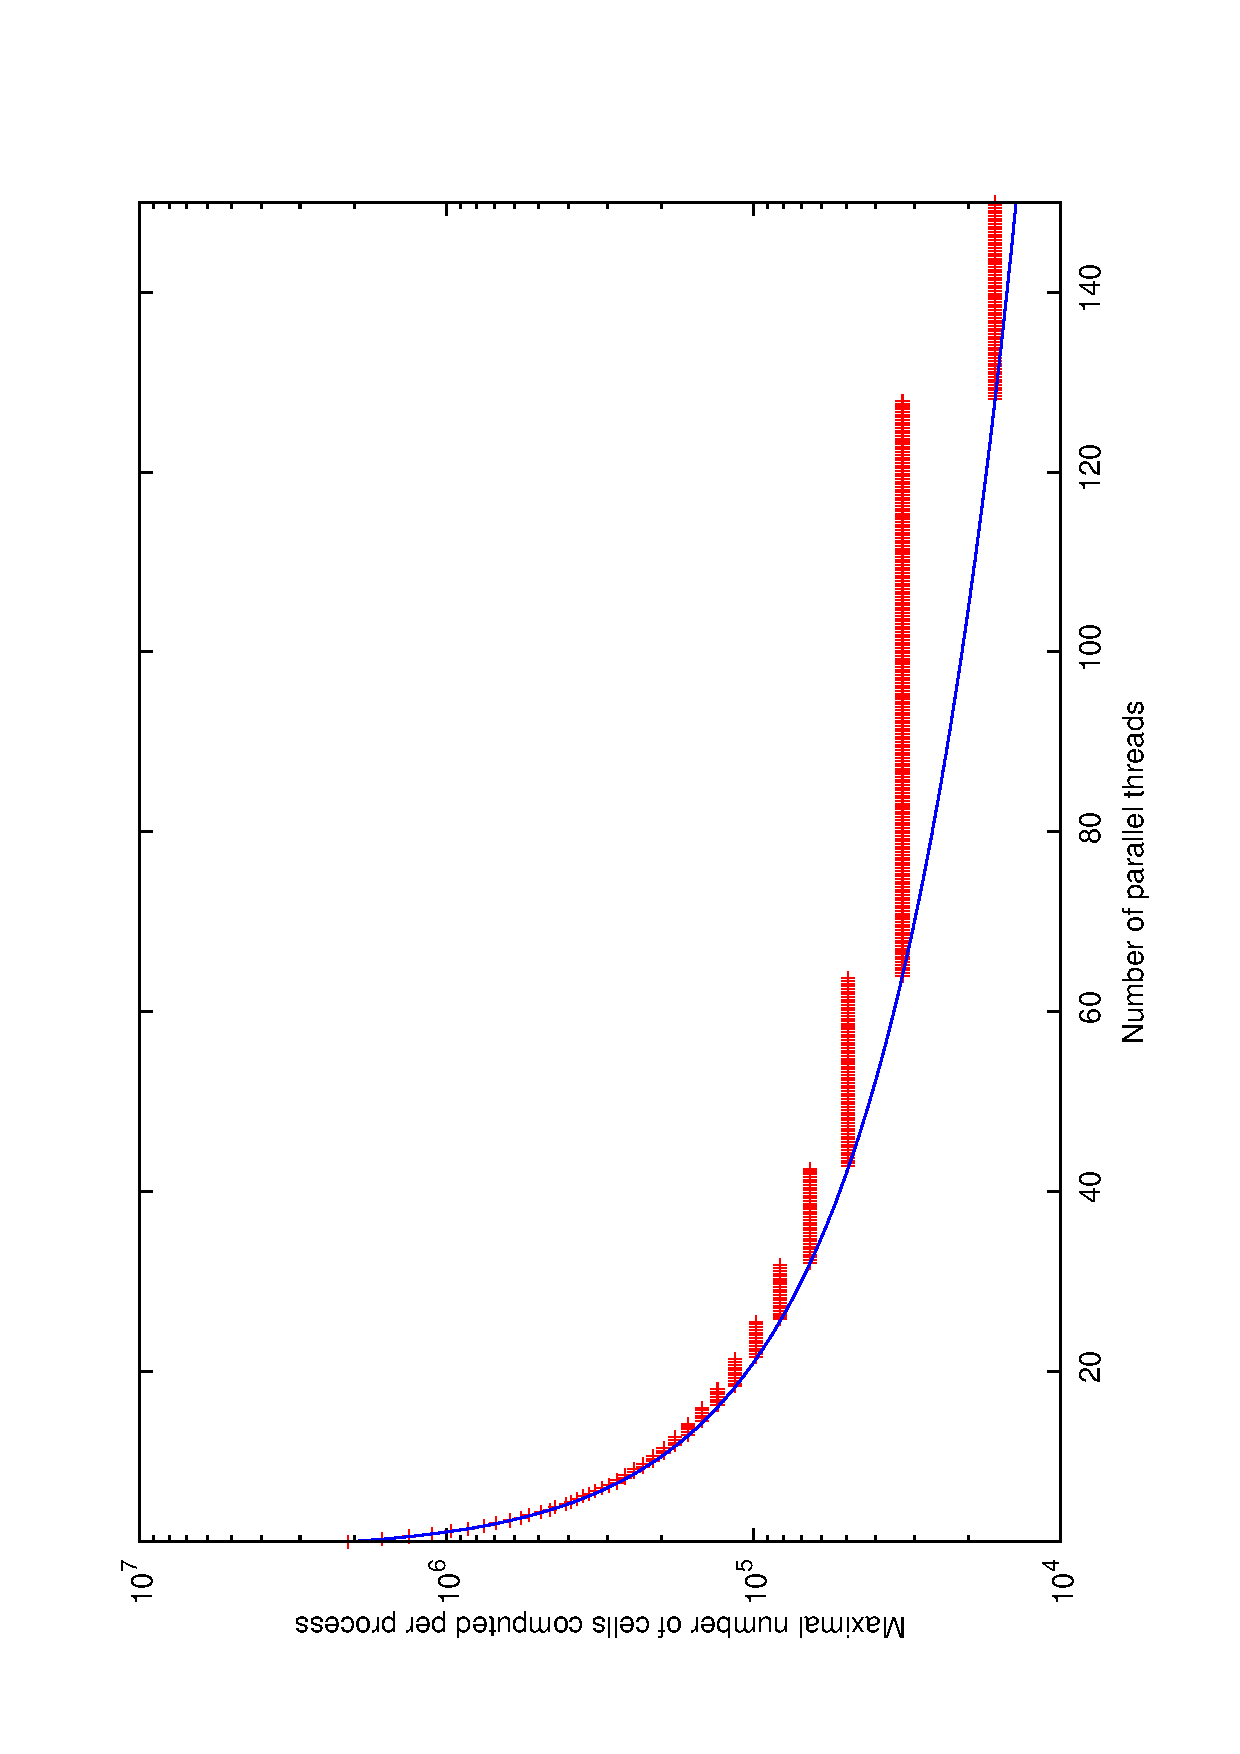
\includegraphics[width=0.5\textwidth, angle =-90]{max_per_thread}
\end{center}
\caption{The position of the crosses corresponds to the maximal number of grid 
cells whose properties have to be computed by a individual thread as a function 
of the number of parallel process. As all cells with the same $z$-index are 
always computed by the same process, the maximal amount of grid cells that has 
to be computed by an individual process is no longer indirectly proportional to 
the number of parallel processes if the number of parallel processes is not 
small compared to the number of cells along the $z$-axis. For comparison, the 
blue line shows an ideal scaling behavior.} \label{fig:maxperthread}
\end{figure}

  
\subsection{Tests}
To test how the run time of our program scales with the number of parallel 
processes we have repeated the same simulation with 1 to 12 parallel 
processes\footnote{The test have been performed on a workstation with 12 
physical cores. So we have chosen 12 as the maximal number of parallel 
processes.}. The test simulation consists of a box with $41^3$ cells, a 
simulated volume of $(31\,\mathrm{pc})^3$ a homogeneous hydrogen number density 
of $10\,\mathrm{cm^{-3}}$ and a chemical composition that corresponds to the 
solar values. As ionizing source we have chosen a $40\,\mathrm{kK}$ dwarf 
model with solar metallicity. The radiation field of 
the stars has been split into $196\,608$ rays.  The simulation included 
computation of the temperature structure of the gas and the ionization structure 
of the contained metals. The simulated time was $30\,000\,\mathrm{yrs.}$. In 
each of our runs, the simulation was finished after 23 iteration steps 
\footnote{We started with a fully ionized H\,II region which allows for larger 
timesteps.}. In Fig.~\ref{fig:performanceplot} we show the execution speed of 
the simulation (in units of iteration cycles per hour of wallclock time) as a 
function of the number of threads and compare it with the ideal case of a 
performance that scales linearly with the number of threads. In 
Fig.~\ref{fig:efficiencyplot} we show the efficiency, i.e. the quotient of the 
measeured and the ideal performance. We find that the efficency drops to 
approximately 90\,\% when the number of processes is increased from 1 to 2. In 
the range from 2 to 12 processes the efficiency decreases more slowly until a 
value of approximately
80\,\% is reached. 

\begin{figure}
\begin{center}
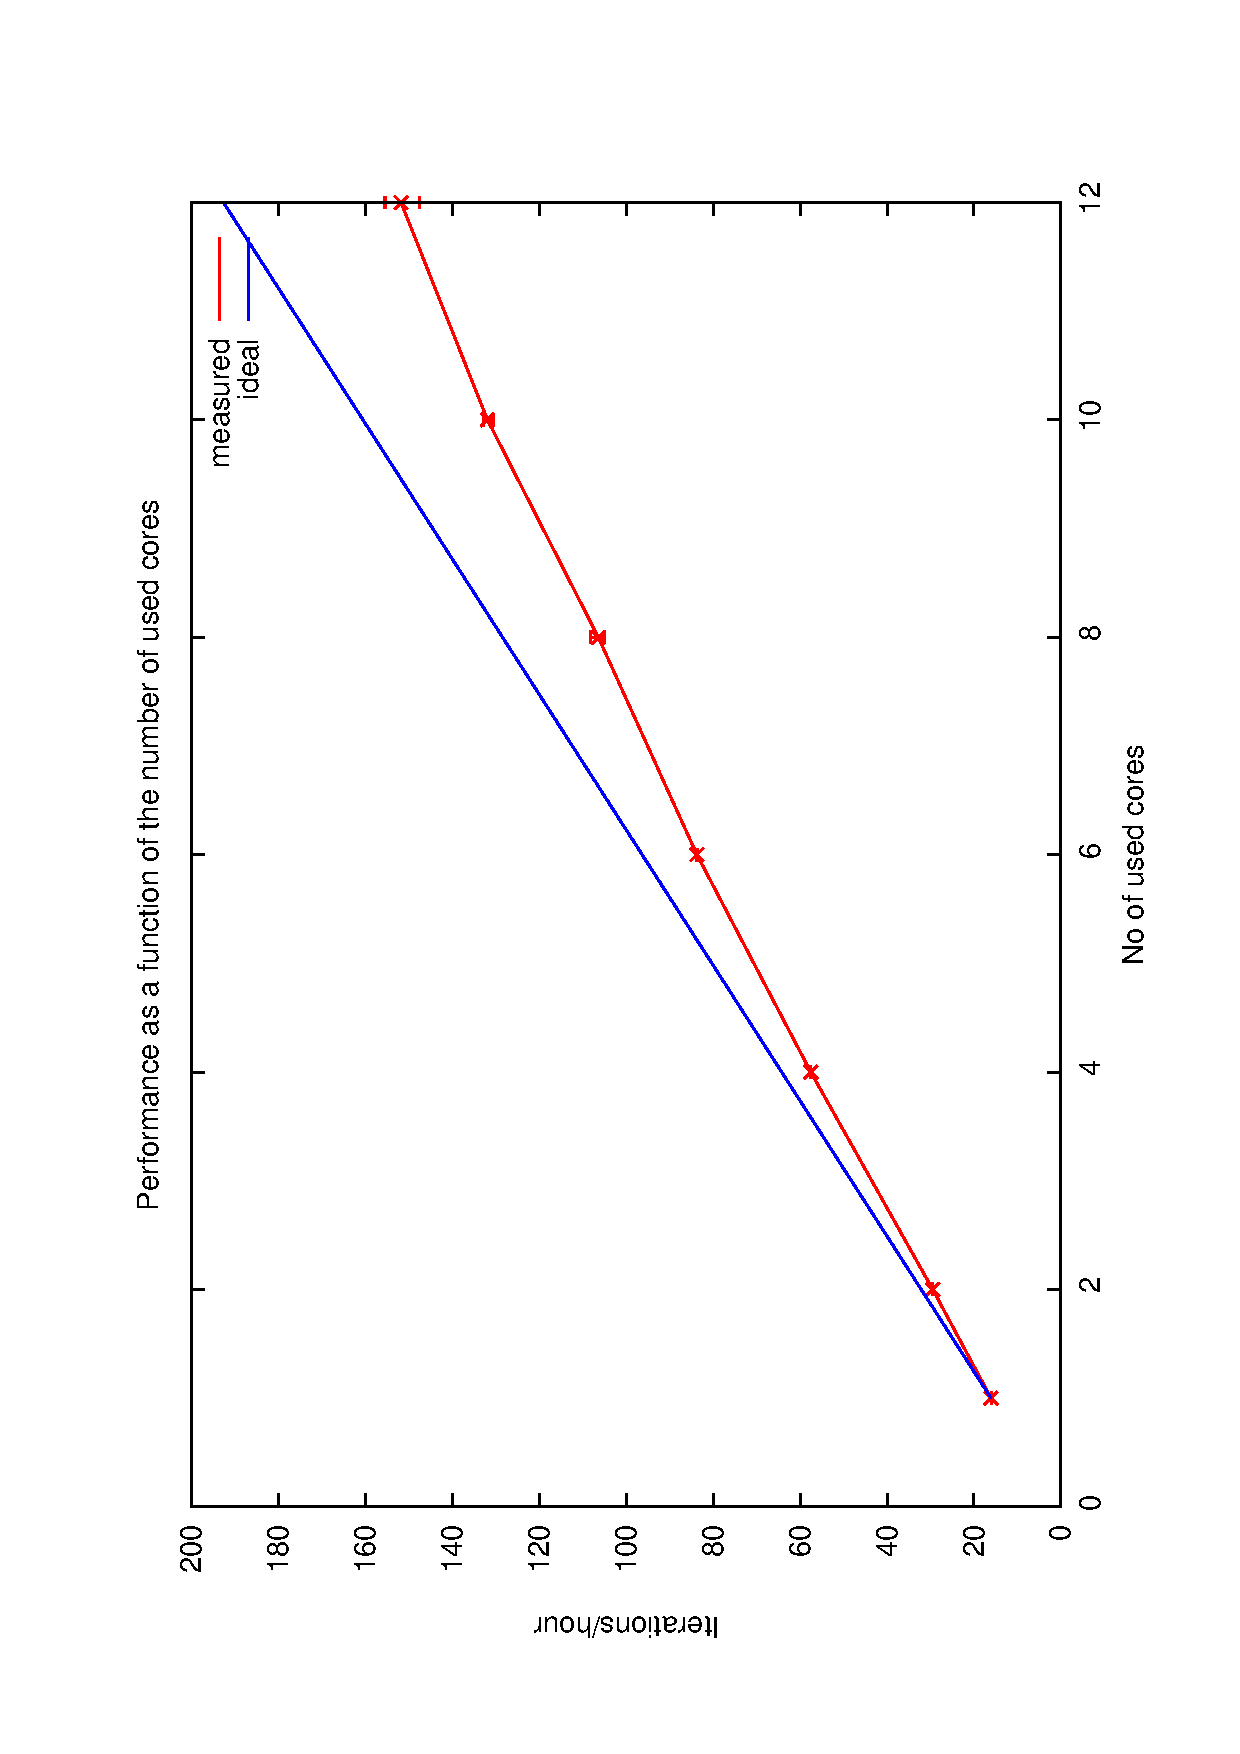
\includegraphics[width=0.5\textwidth, angle =-90]{performanceplot}
\end{center}
\caption{Performance of the simulation in iteration cycles per hour as a 
function of the number of computing threads. The red line shows the measured 
values. For the measurements with at least parallel processes we have performed 
several runs. In the case of 12 processes we found variations of the run time of 
approximately 2\,\%. The blue lines shows a linear scaling of the performance 
for one process with the number of processes, which would describe the 
performance for an ideal parallelization.
} 
\label{fig:performanceplot}
\begin{center}
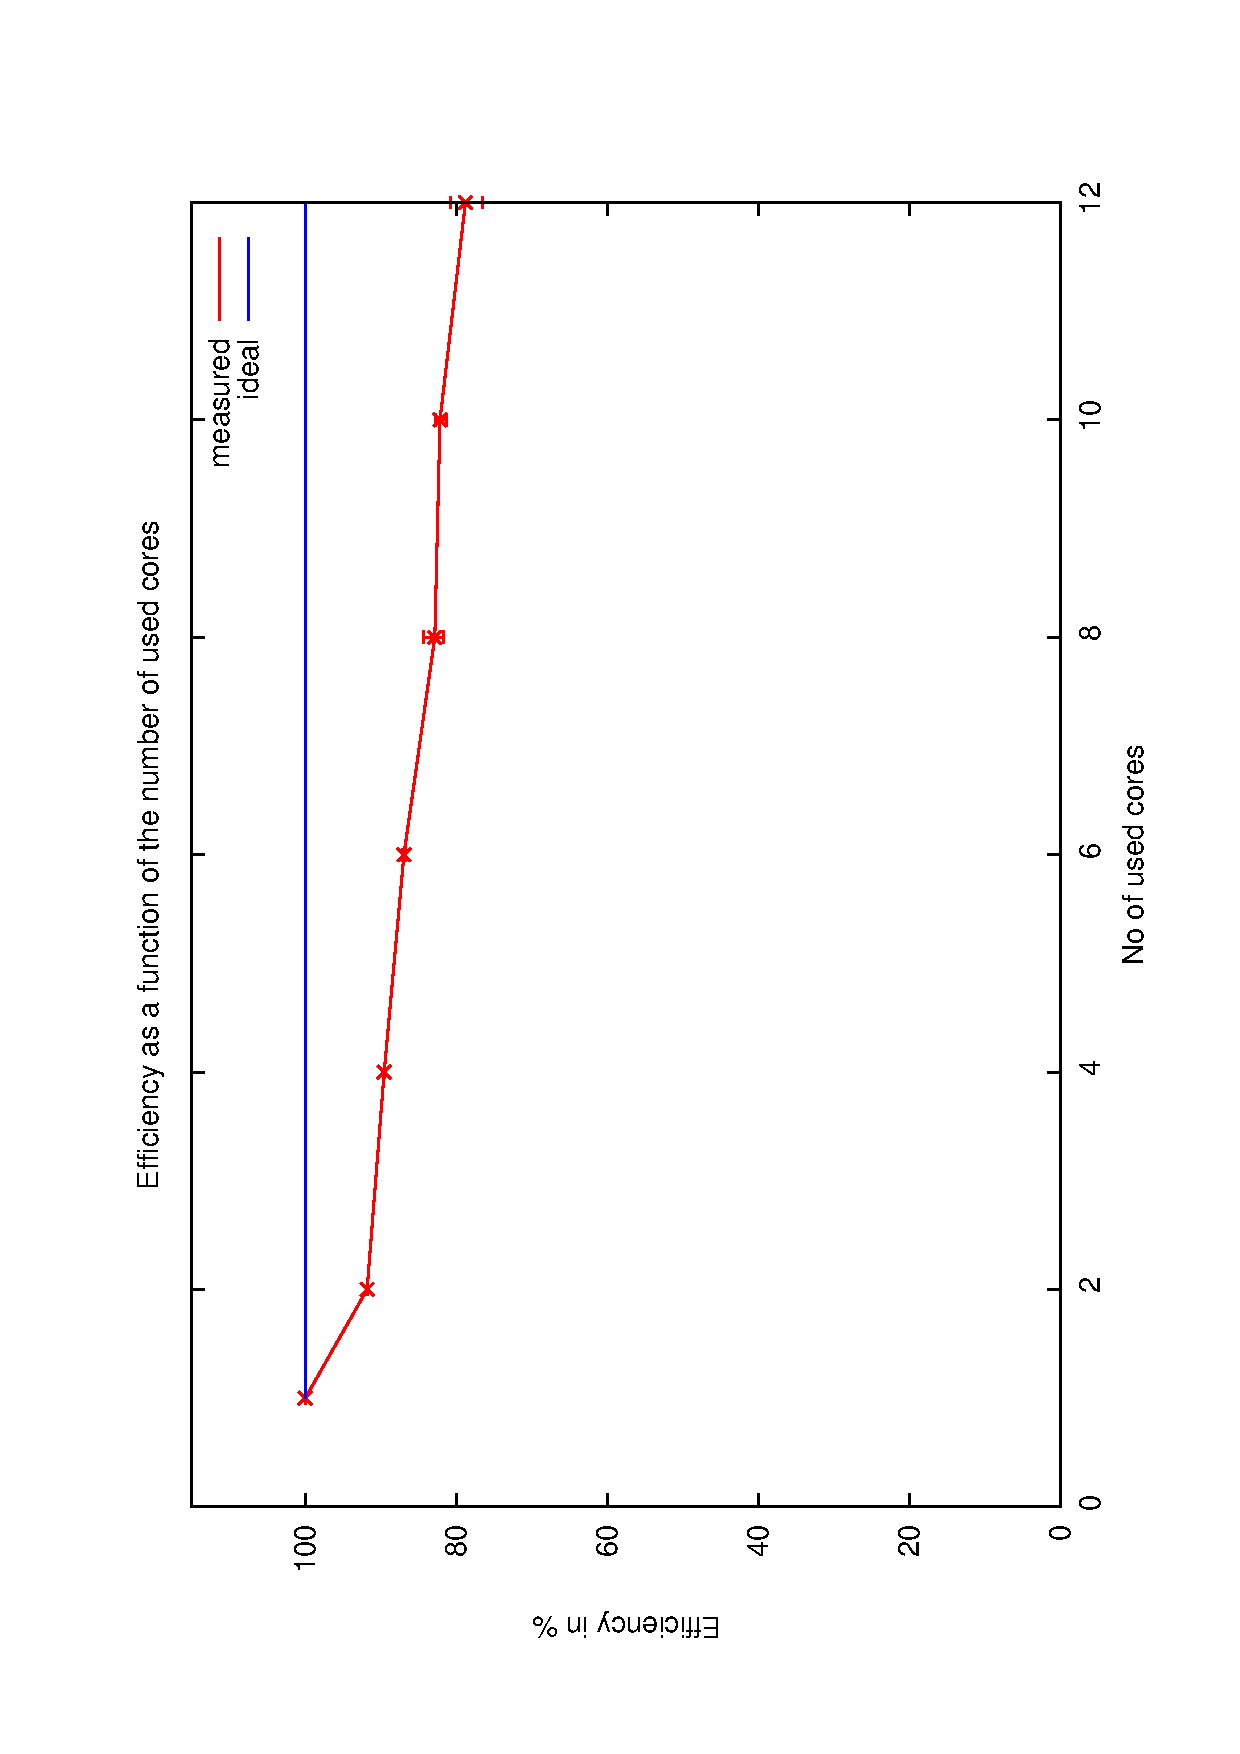
\includegraphics[width=0.5\textwidth, angle=-90]{efficiencyplot}
\end{center}
\caption{The efficiency of the parallelization drops to approximately 80\, \% 
for 12 parallel processes.}
\label{fig:efficiencyplot}
\end{figure}
 
\end{appendix}

\bibliography{manual}
\end{document}          
